\chapter{Засоби формалізації голосової інформації в системах диспетчерського контролю за рухом автотранспорту} \label{chapt4}

\section{Опис розроблених засобів формалізації голосової інформації в системах диспетчерського контролю за рухом автотранспорту} \label{sect4_0}

Для використання розроблених моделей, був створений мобільний додаток для системи Android, оскільки вона є більш розповсюджена, а вартість смартфонів на цій системі нижча, що є важливим для зниження витрат на впровадження системи.

Додаток доступний безкоштовно у системному магазині Google Play і може при бажанні бути встановлений будь-яким водієм на власний Android-смартфон. Назва додатку «Plannary Last Mile».

Оскільки основним способом керування додатком є голосові команди, то візуальний інтерфейс додатку є достатньо простим. В загальному вигляді інтерфейс складається з вікна налаштувань (рис. \ref{img:app-opt}), вікна загальної інформації про маршрут (рис. \ref{img:app-info}), маршрутного листа (рис. \ref{img:app-list}), мапи маршруту (рис. \ref{img:app-map} та \subcaptionref{img:app-map-late}) та вікна інформації про точку (рис. \ref{img:app-point}).

\begin{figure}
	\centering
	\hspace{0pt plus1fill}
	\subbottom[\label{img:app-no1}]{%
		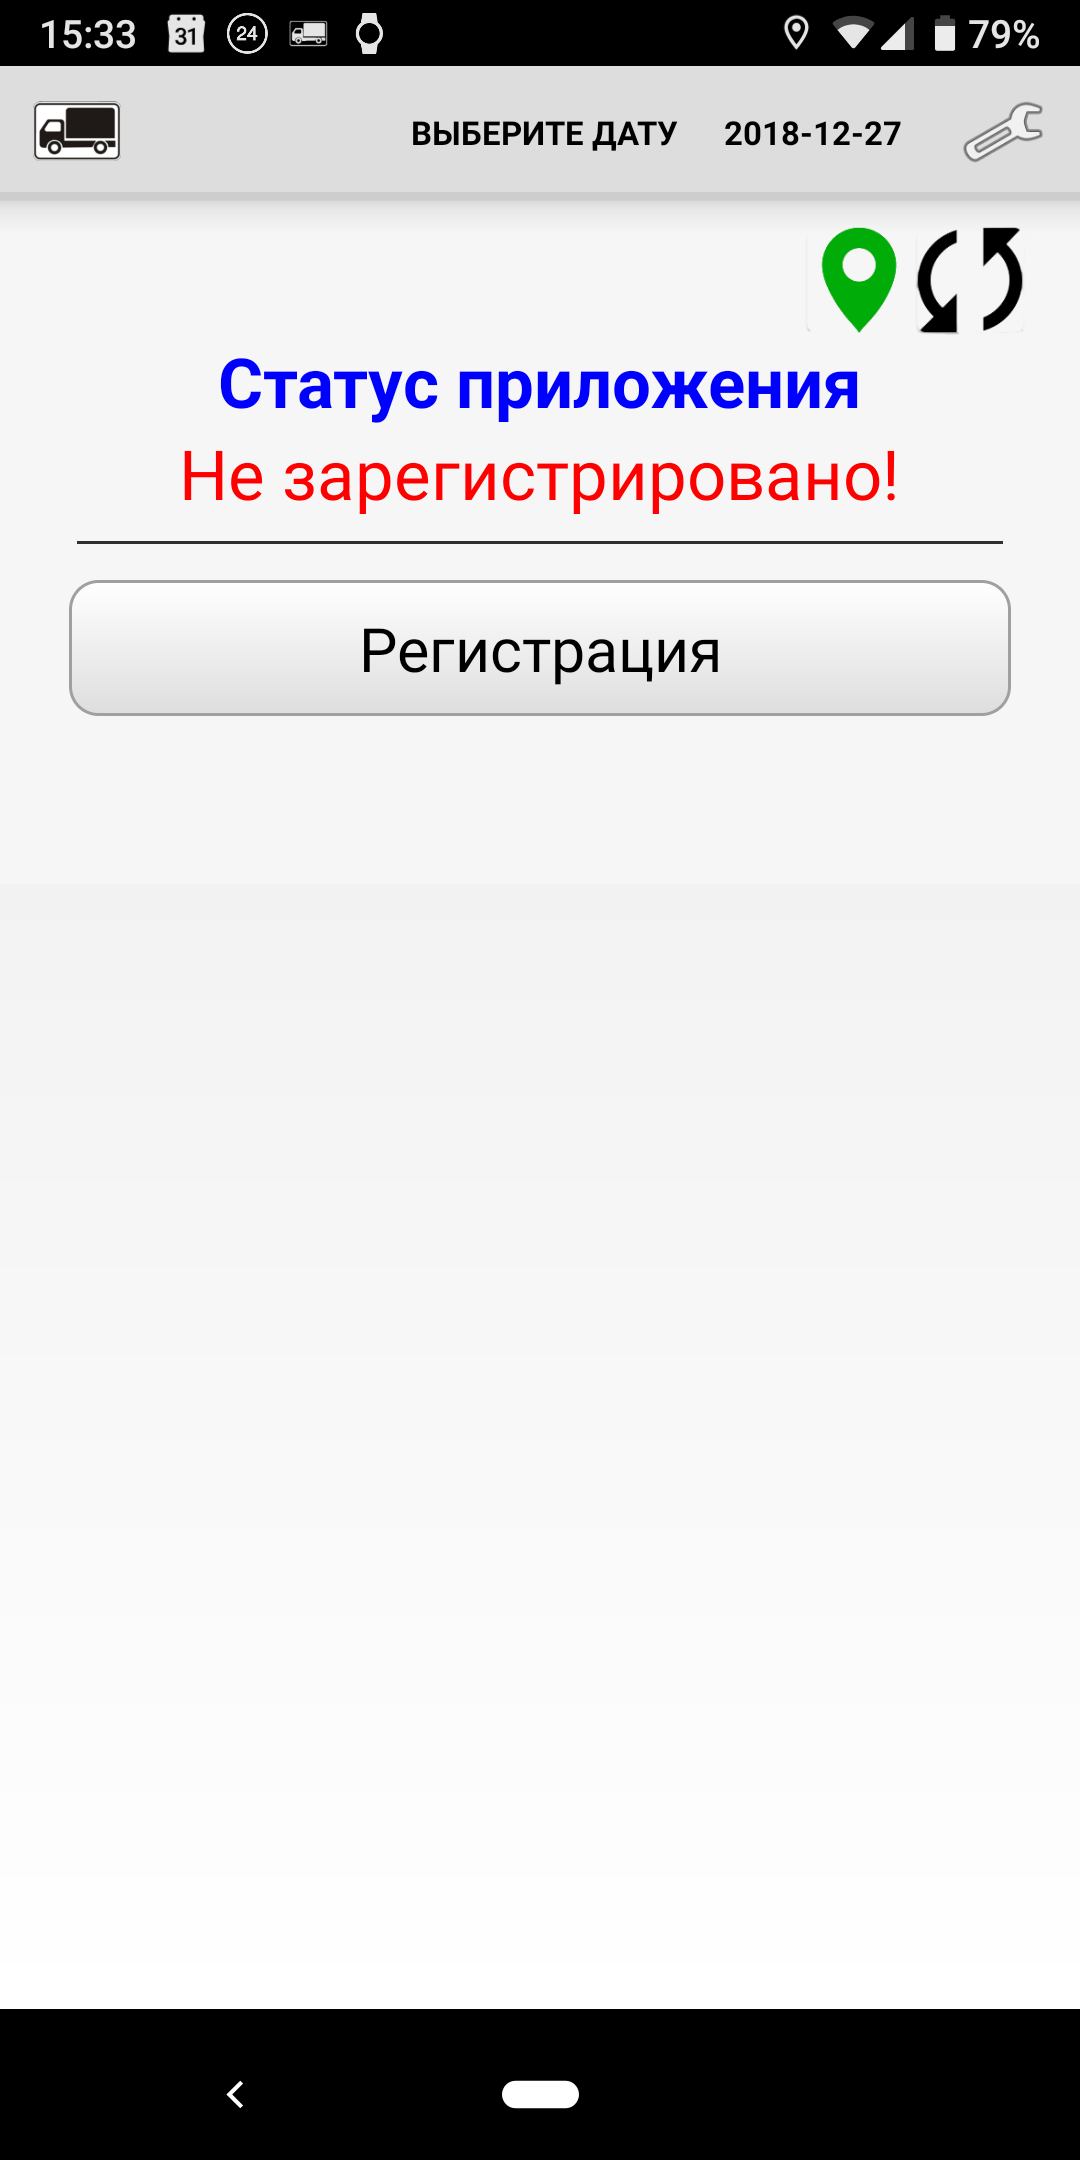
\includegraphics[width=.32\linewidth]{app-no1}}
	\hspace{0pt plus2fill}
	\subbottom[\label{img:app-no2}]{%
		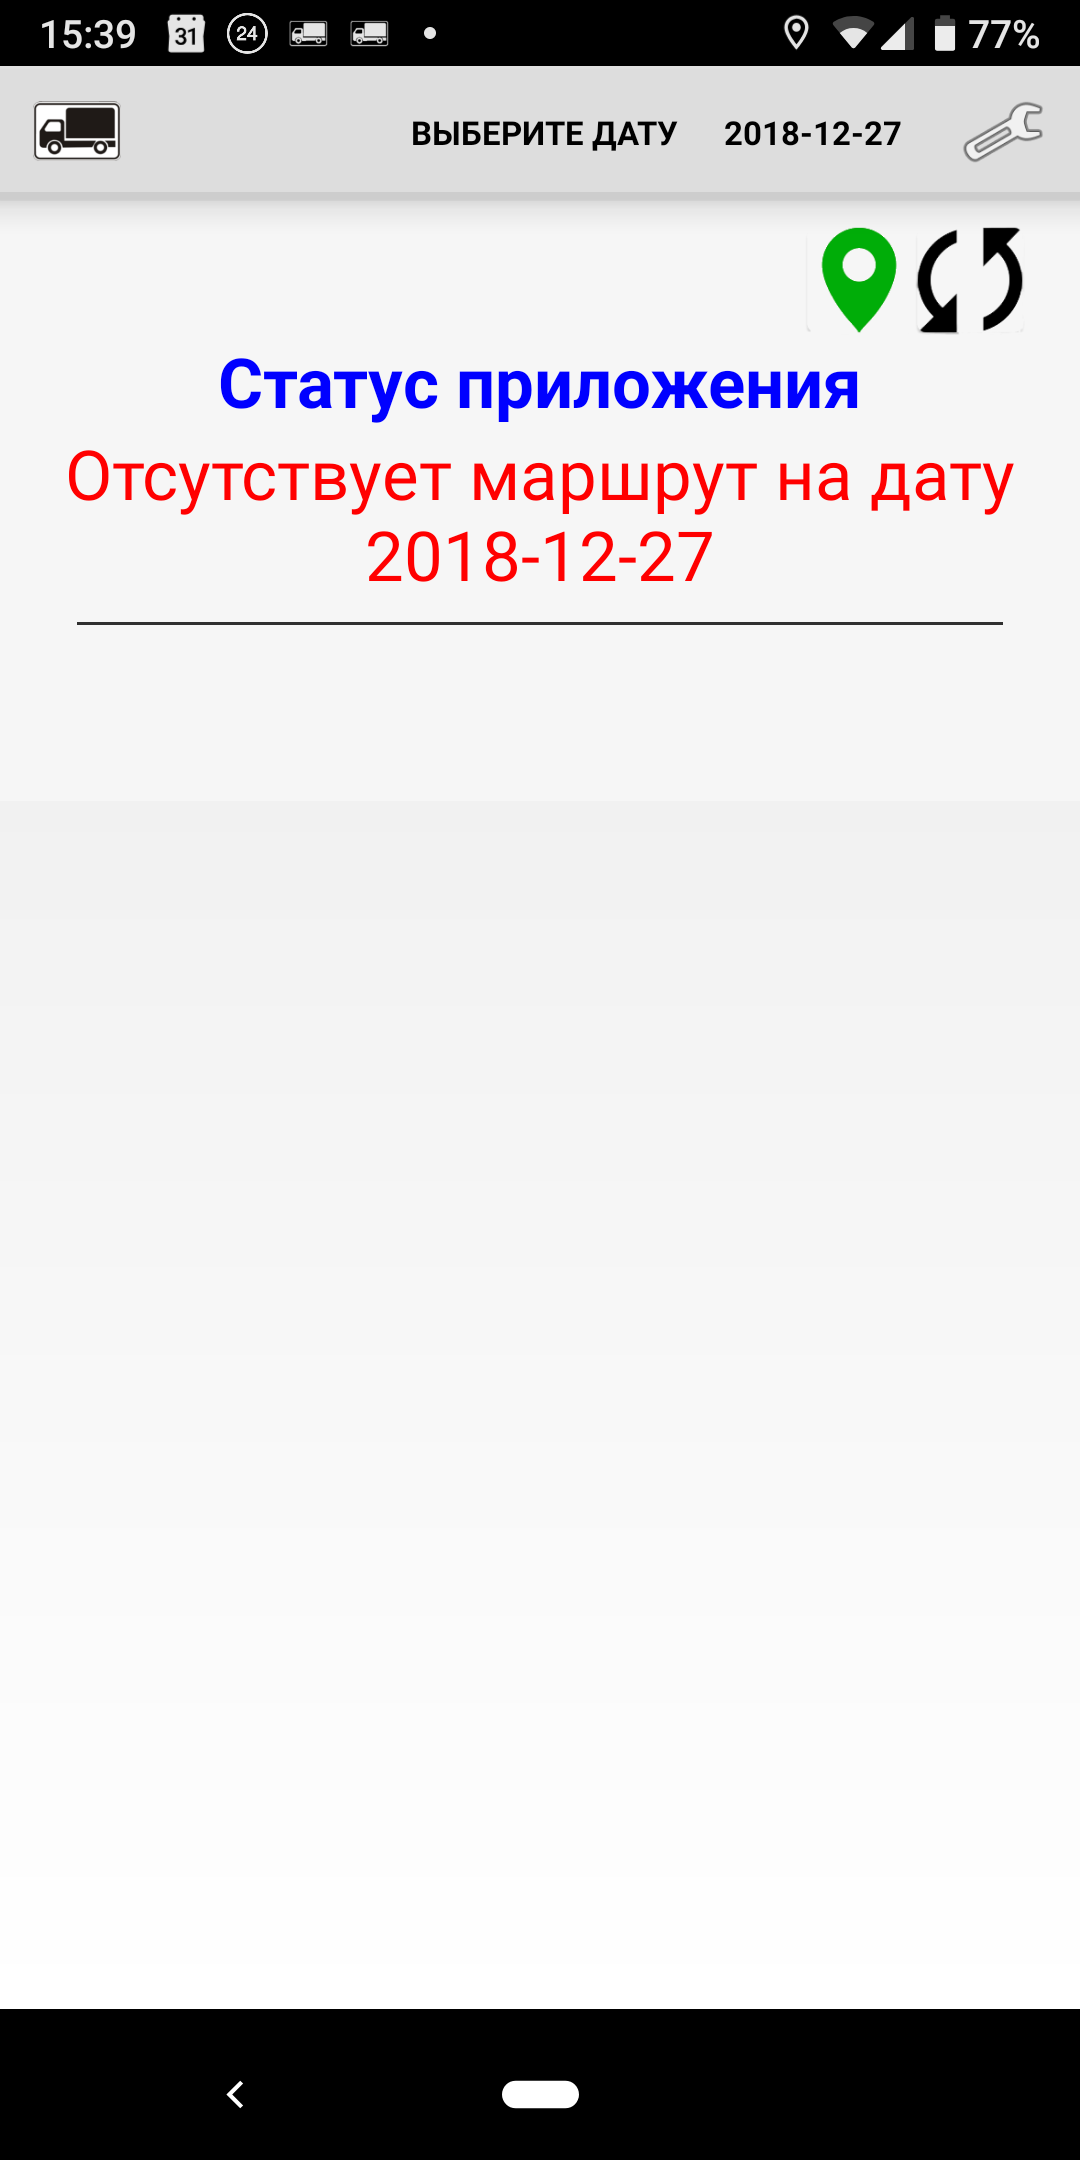
\includegraphics[width=.32\linewidth]{app-no2}}
	\hspace{0pt plus2fill}
	\subbottom[\label{img:app-opt}]{%
		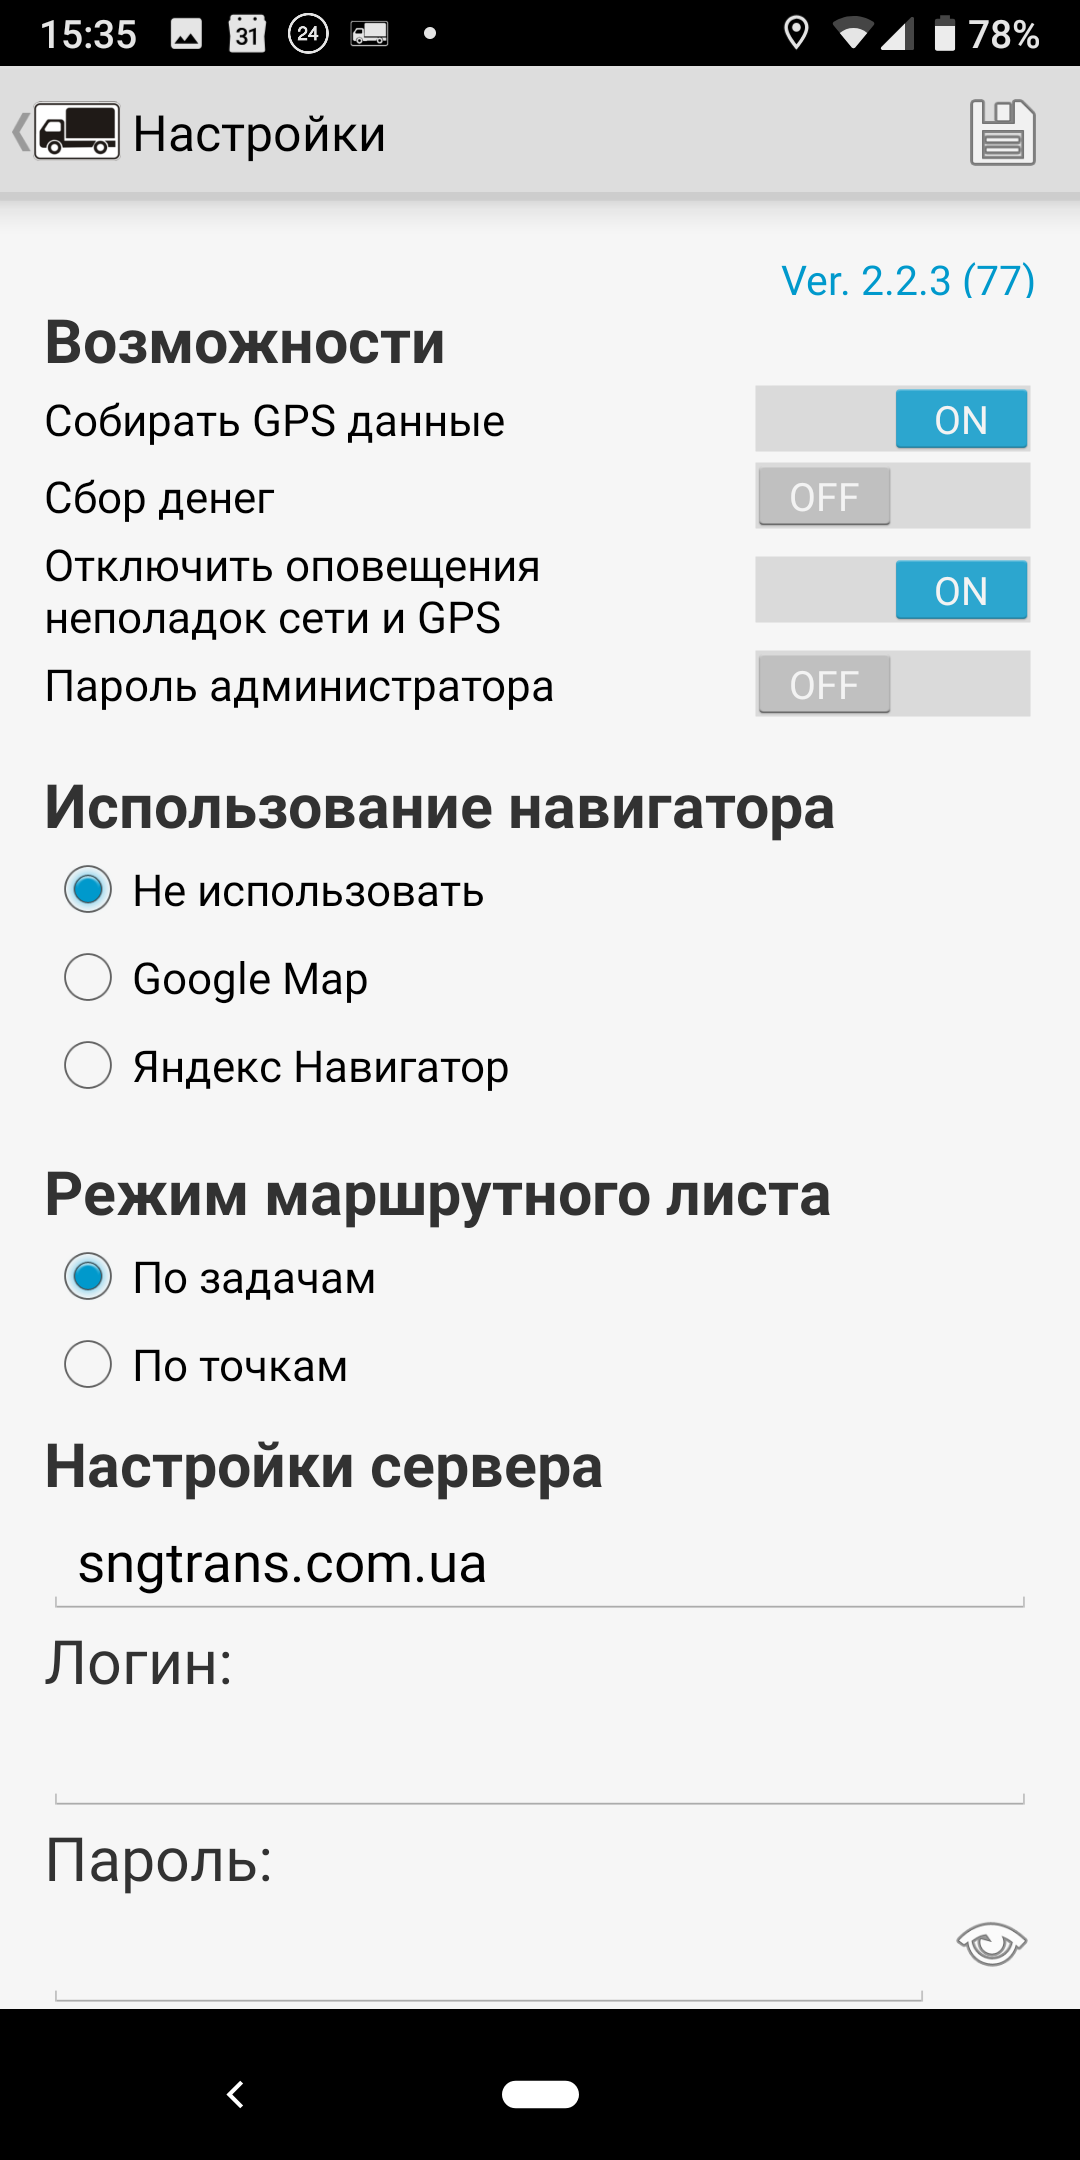
\includegraphics[width=.32\linewidth]{app-opt}}
	\hspace{0pt plus1fill}
	\caption{Вигляд інтерфейсу додатка для незареєстрованого пристрою (\subcaptionref{img:app-no1}), для випадку коли маршрут на вибрану дату відсутній (\subcaptionref{img:app-no2}) та вікно налаштувань (\subcaptionref{img:app-opt})}
	\label{img:app-base}
\end{figure}

\begin{figure}
	\centering
	\hspace{0pt plus1fill}
	\subbottom[\label{img:app-info1}]{%
		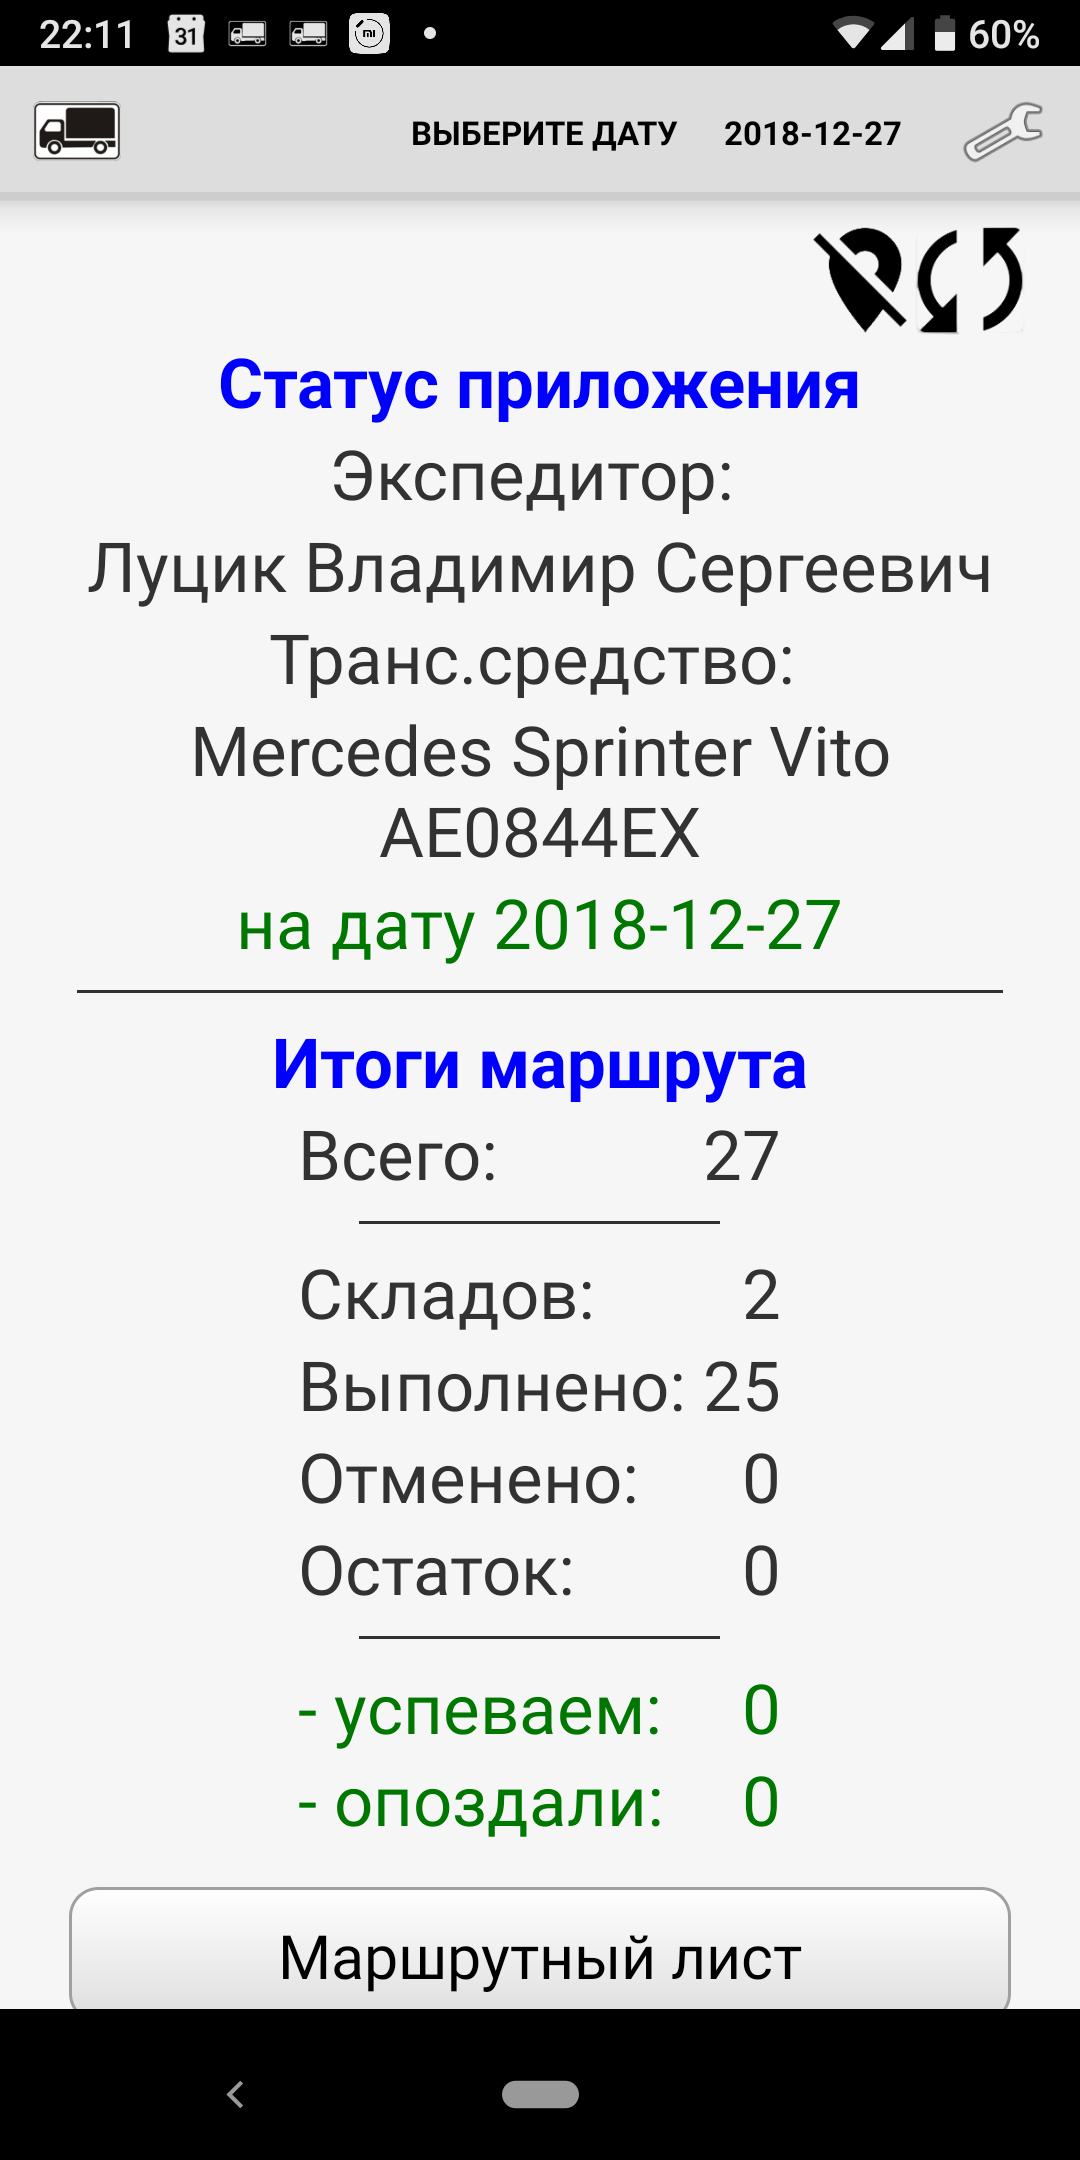
\includegraphics[width=.32\linewidth]{app-info1}}
	\hspace{0pt plus2fill}
	\subbottom[\label{img:app-info2}]{%
		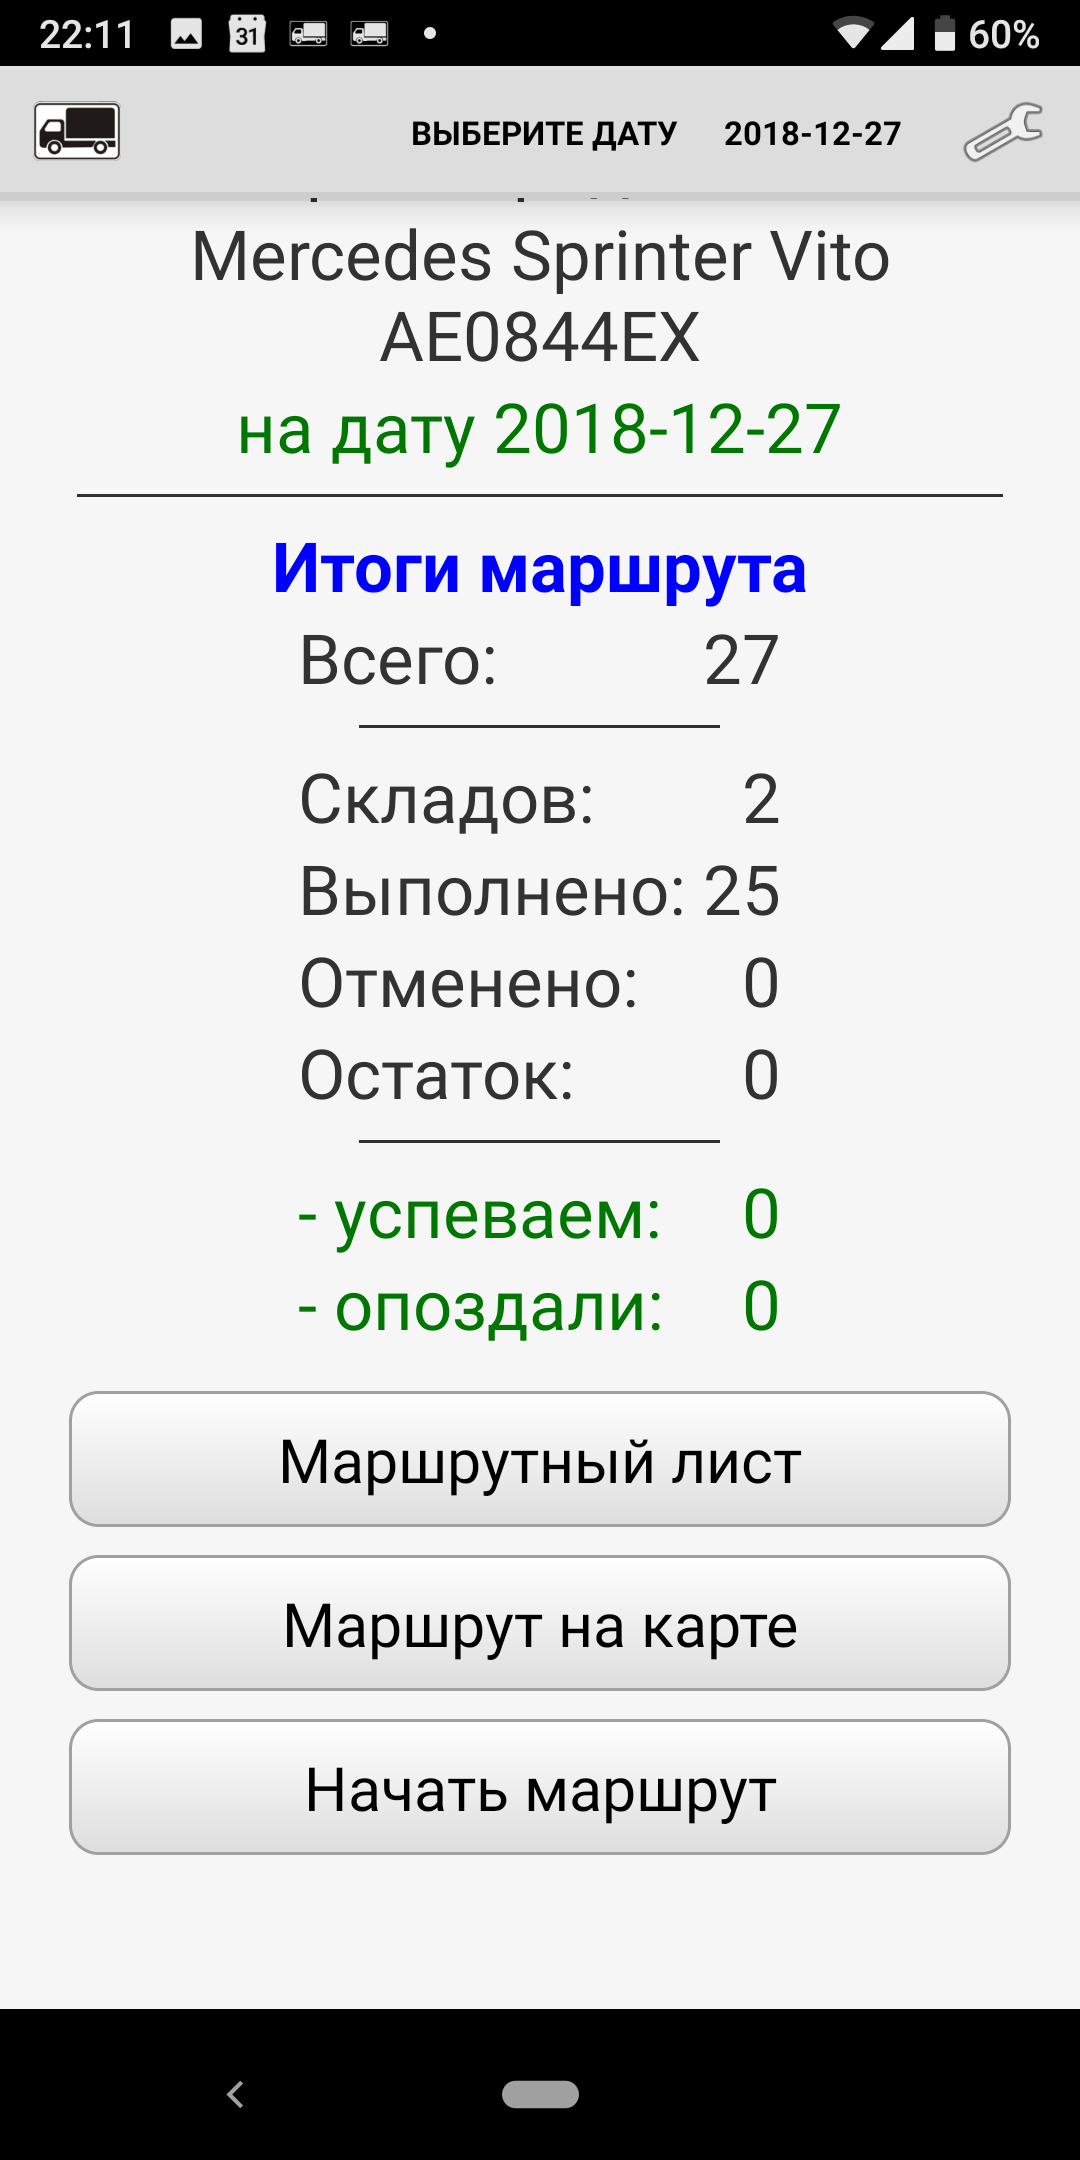
\includegraphics[width=.32\linewidth]{app-info2}}
	\hspace{0pt plus2fill}
	\subbottom[\label{img:app-info-late}]{%
		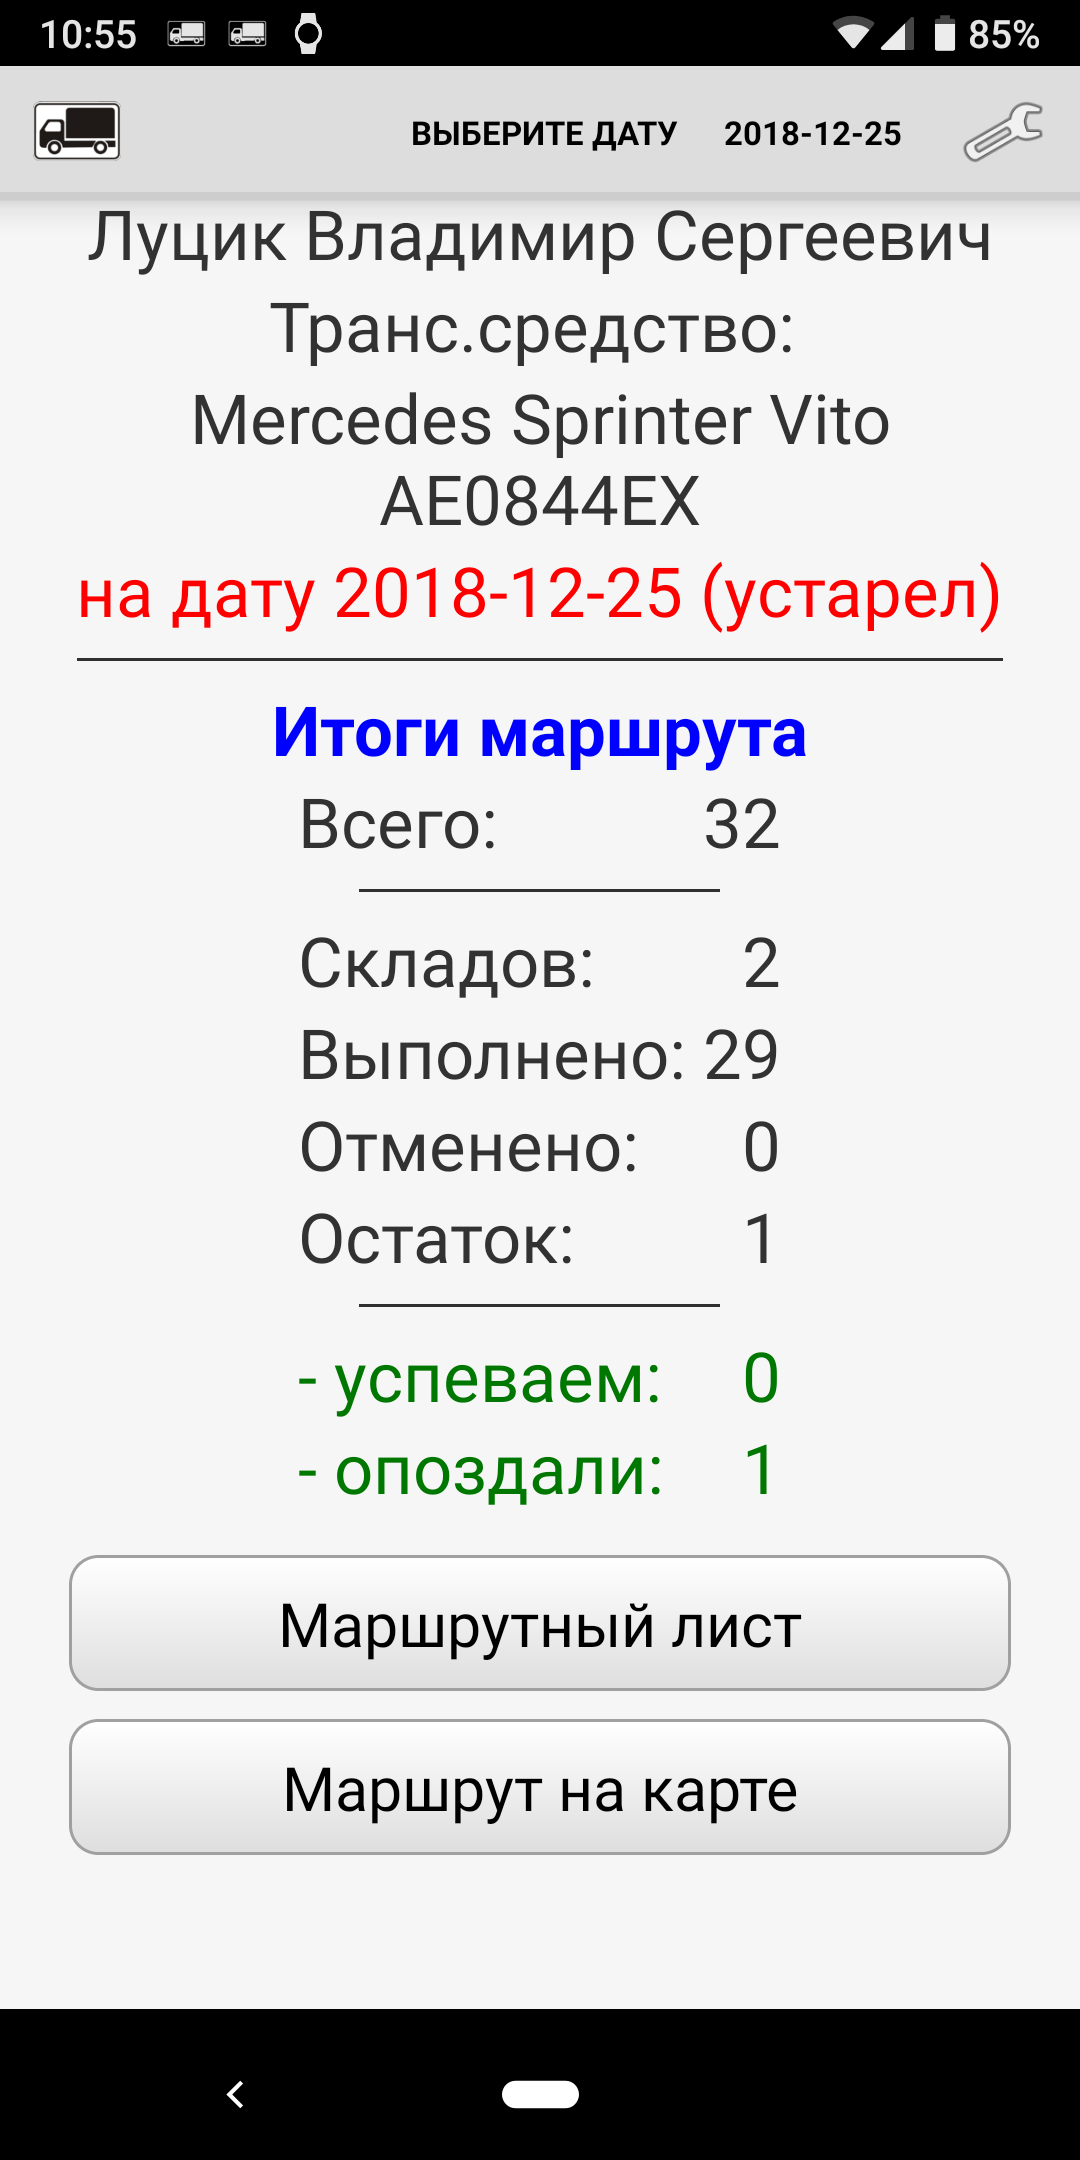
\includegraphics[width=.32\linewidth]{app-info-late}}
	\hspace{0pt plus1fill}
	\caption{Інтерфейс загальної інформації про маршрут, в тому числі з відміткою не виконаних точок (\subcaptionref{img:app-list-late})}
	\label{img:app-info}
\end{figure}

\begin{figure}
	\centering
	\hspace{0pt plus1fill}
	\subbottom[\label{img:app-list1}]{%
		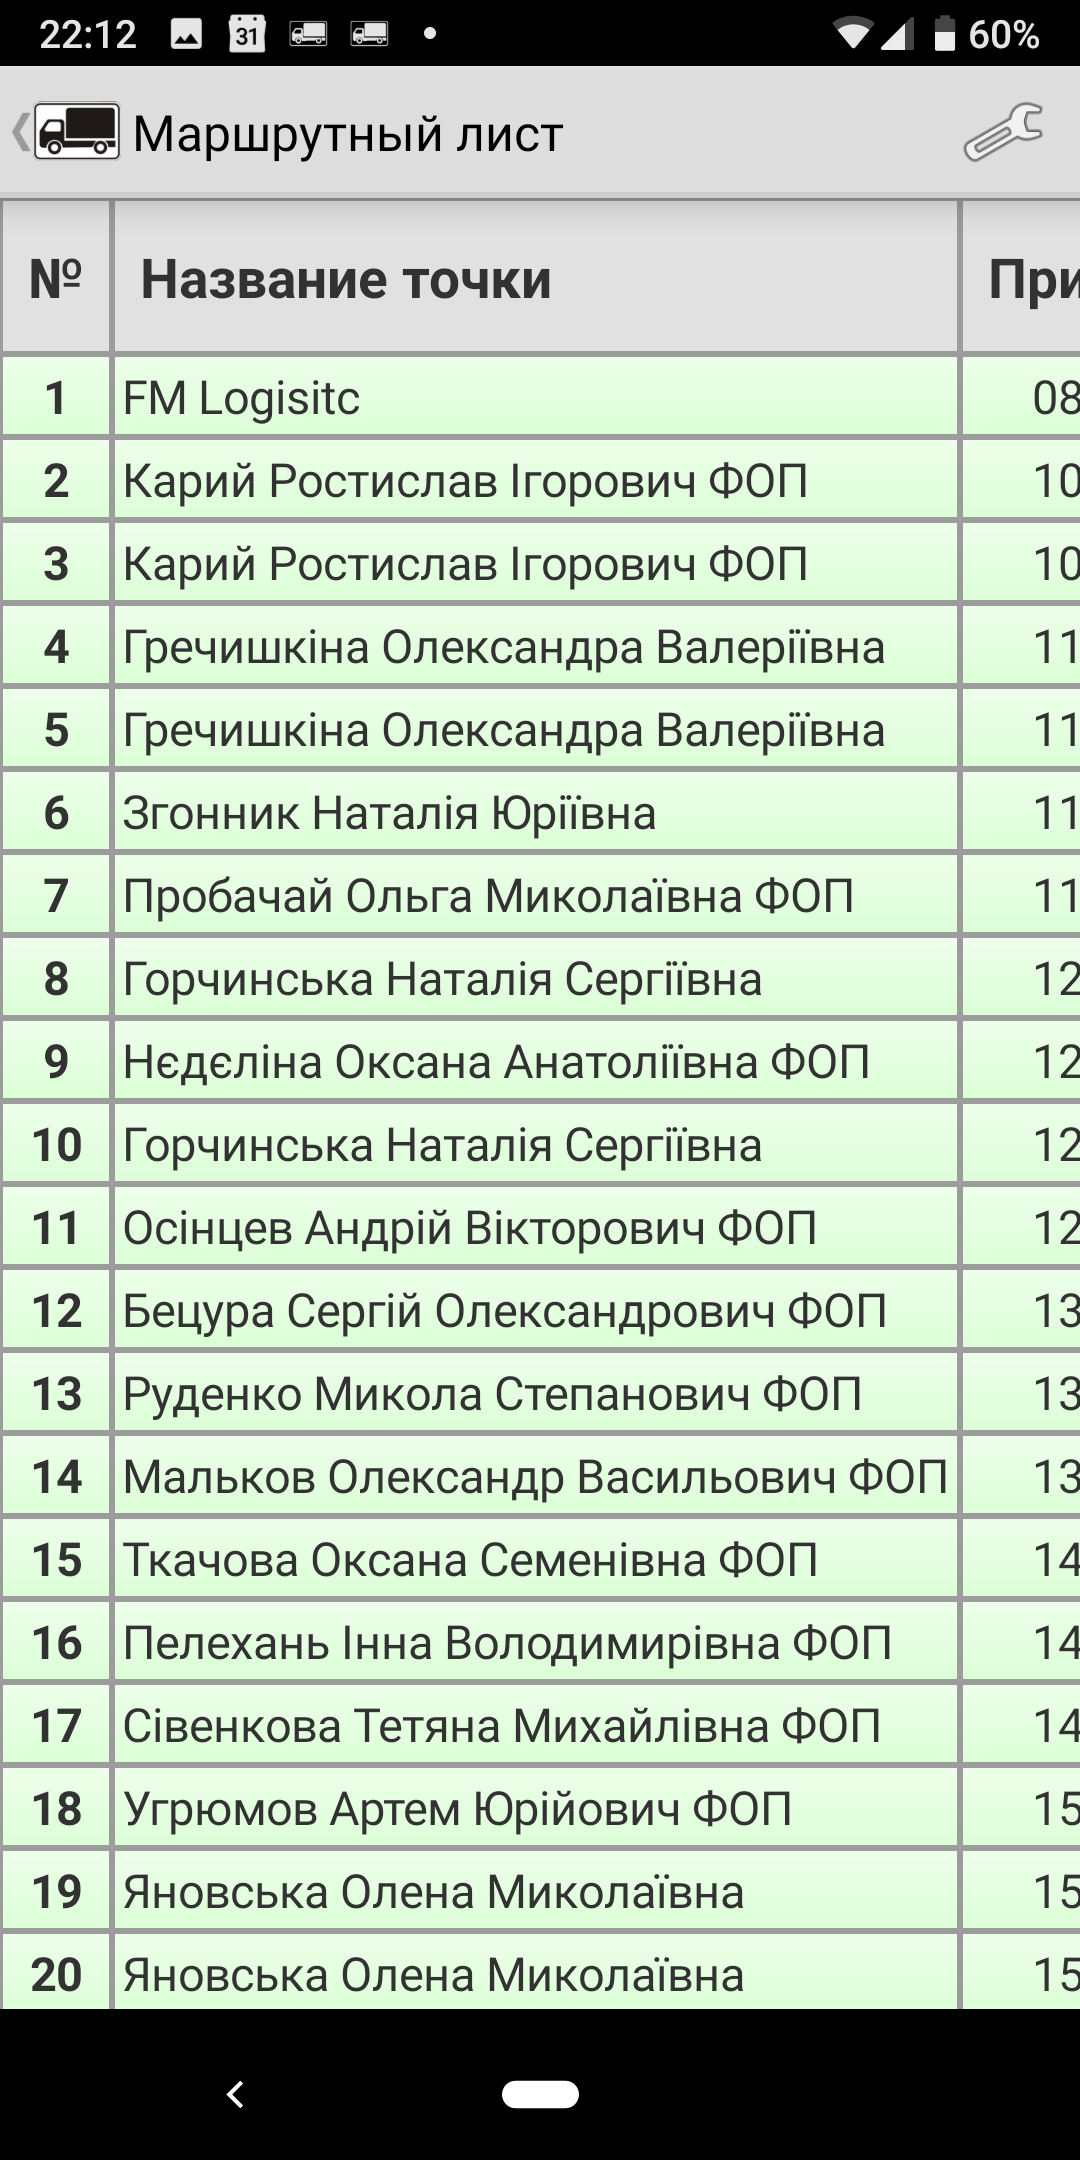
\includegraphics[width=.32\linewidth]{app-list1}}
	\hspace{0pt plus2fill}
	\subbottom[\label{img:app-list2}]{%
		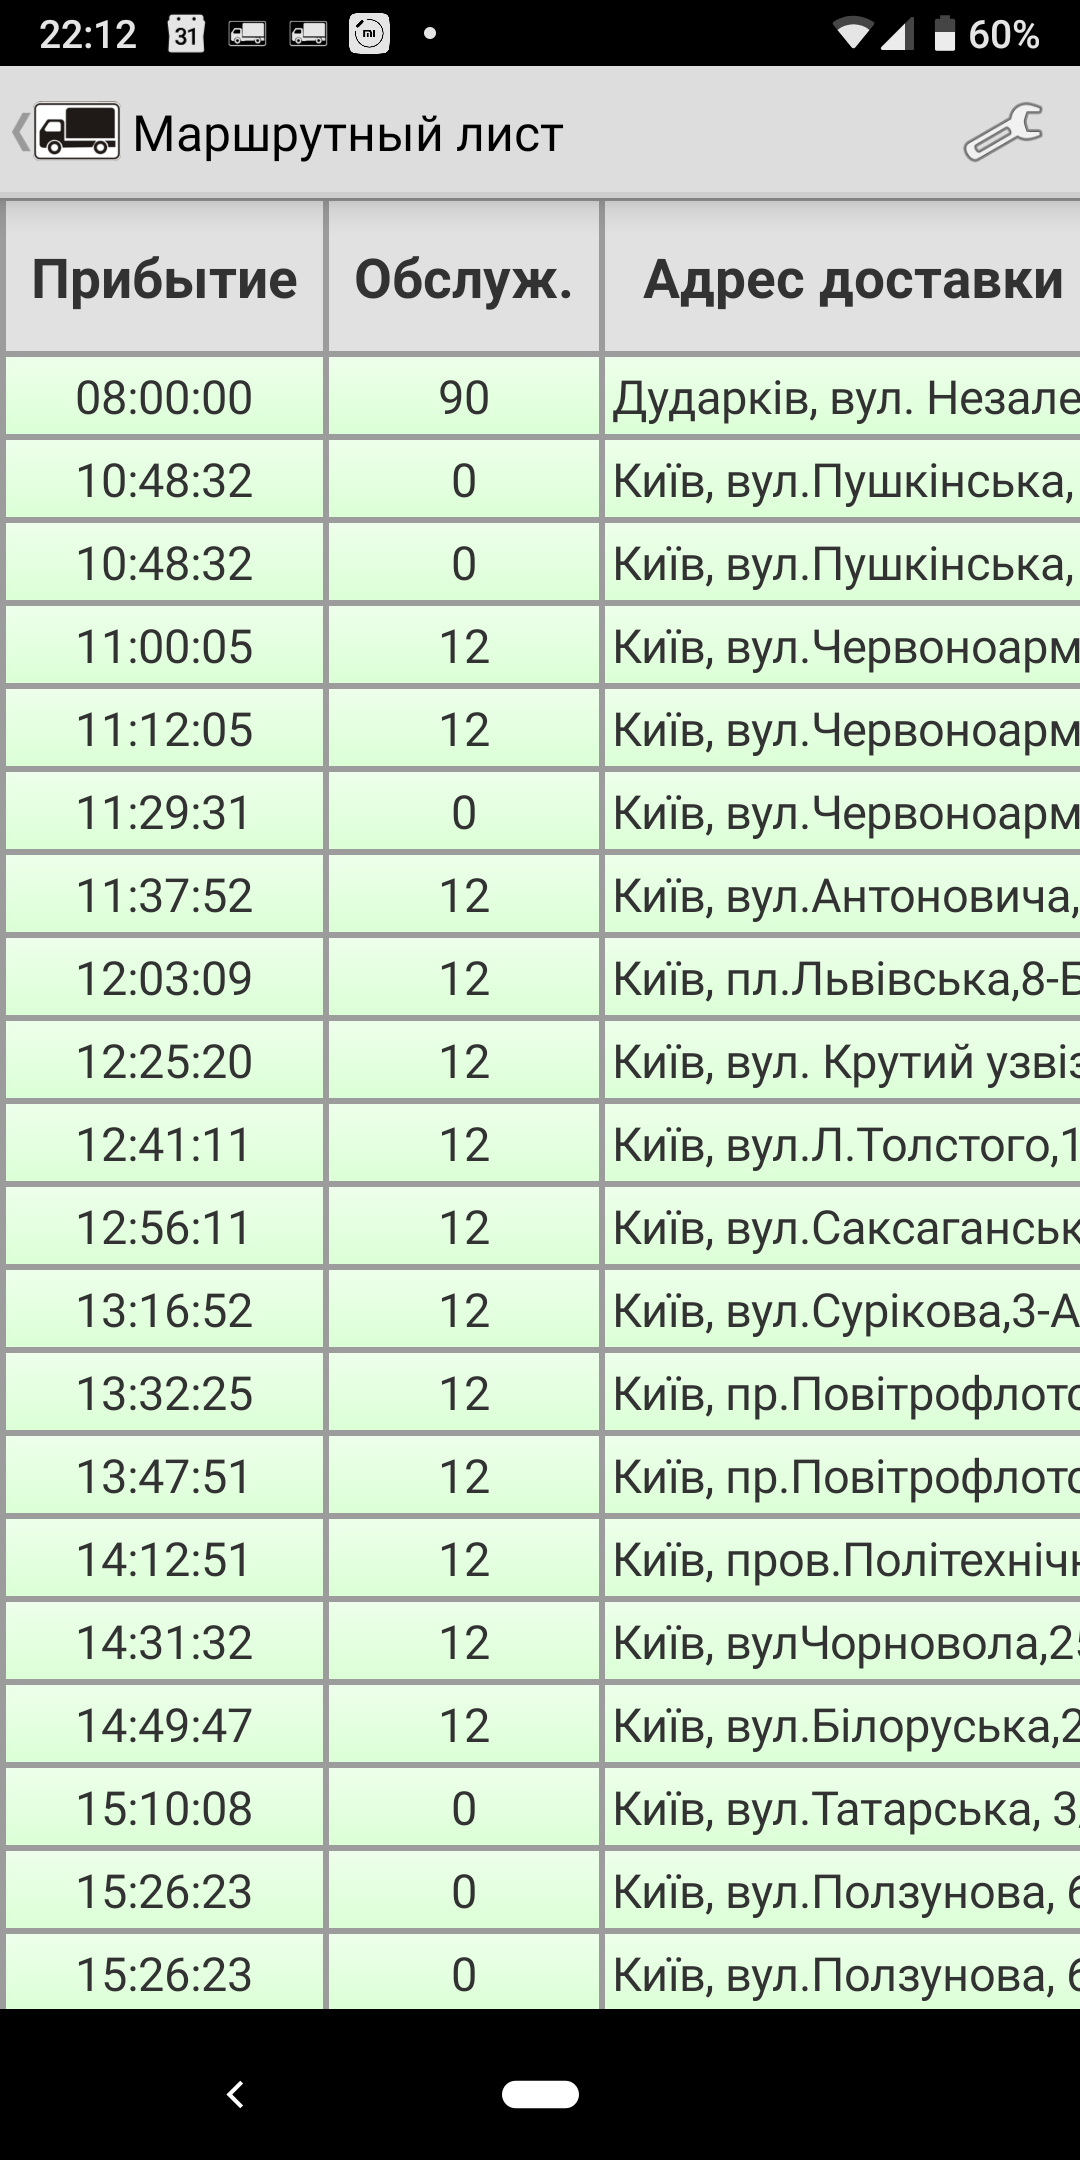
\includegraphics[width=.32\linewidth]{app-list2}}
	\hspace{0pt plus2fill}
	\subbottom[\label{img:app-list-late}]{%
		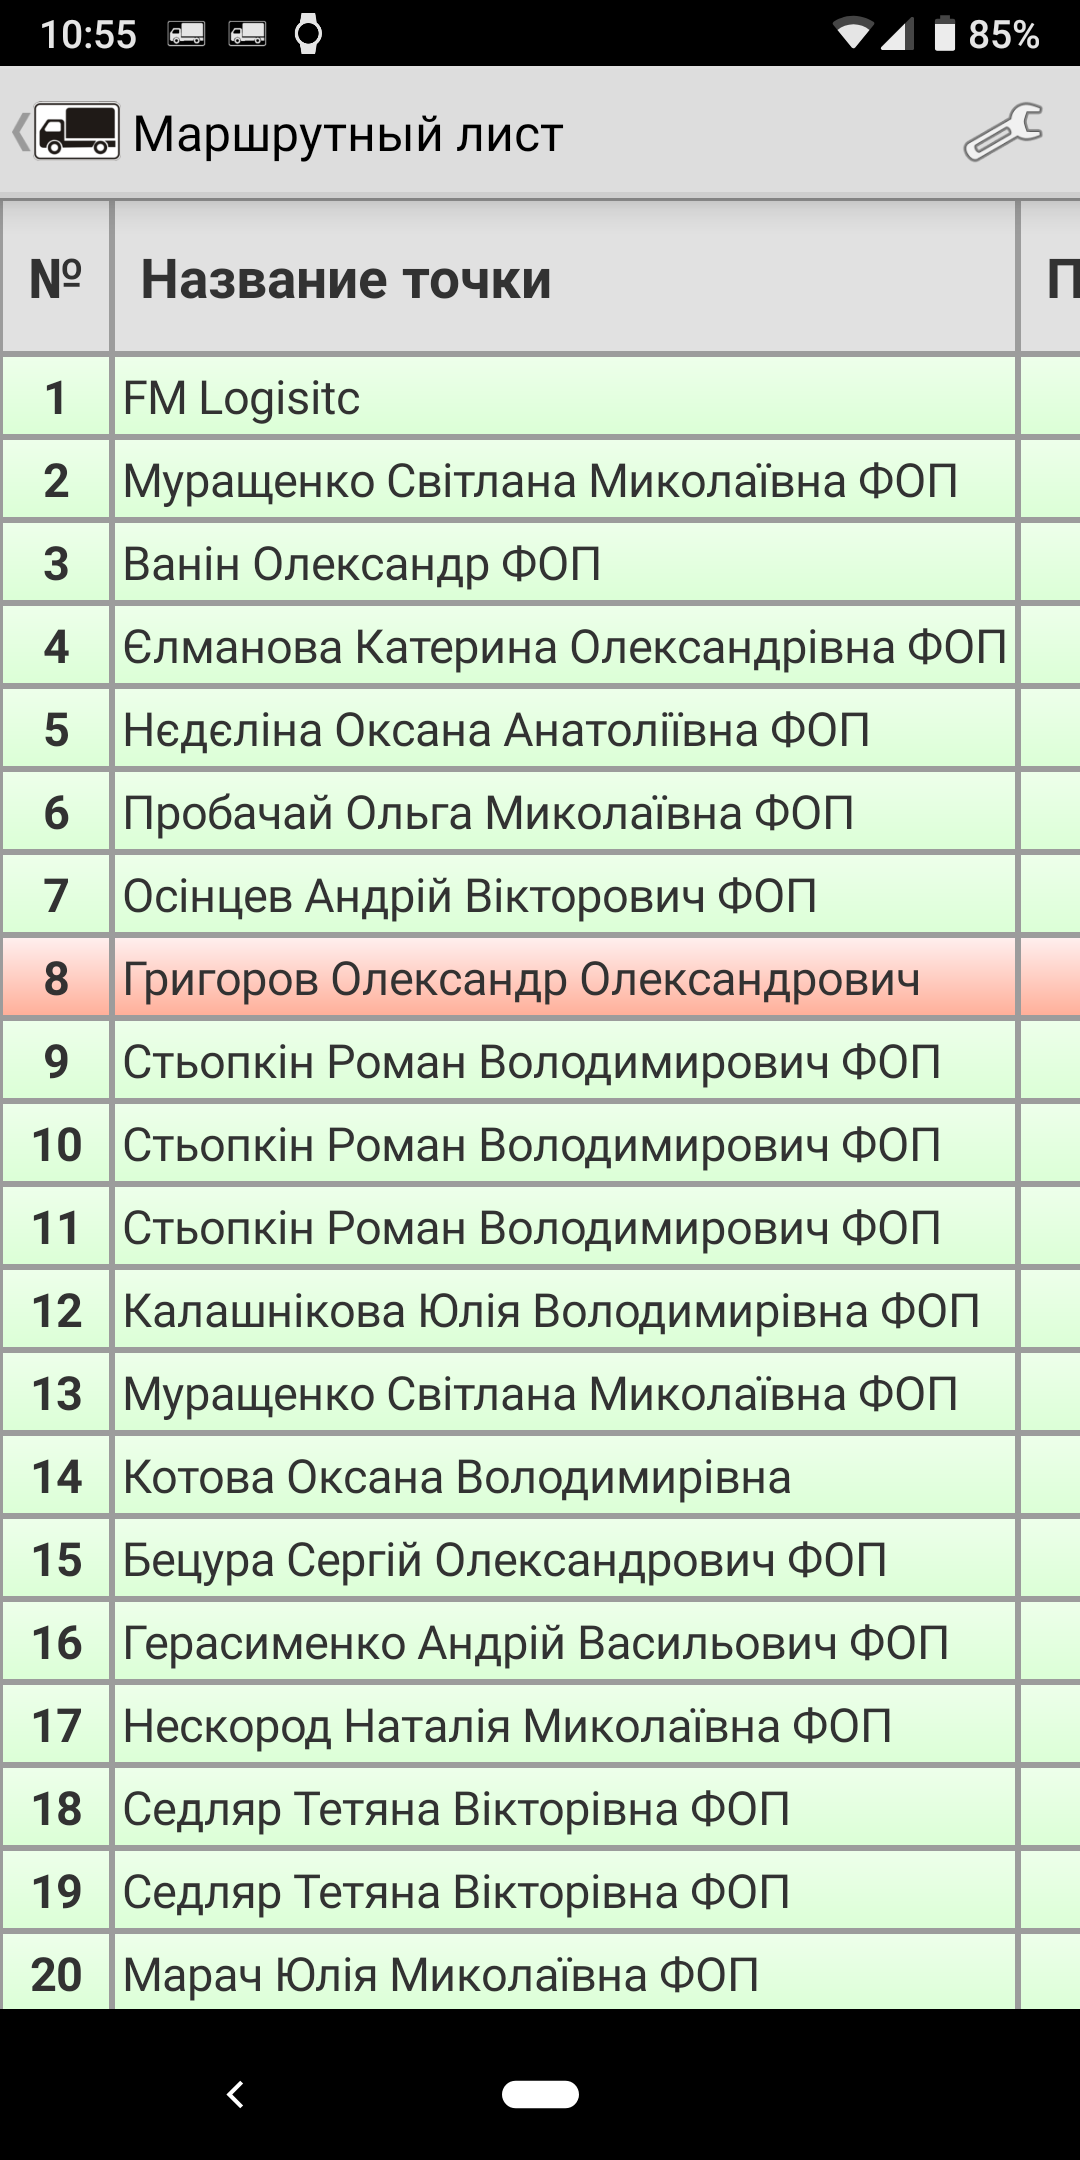
\includegraphics[width=.32\linewidth]{app-list-late}}
	\hspace{0pt plus1fill}
	\caption{Інтерфейс вікна маршрутного листа, в тому числі з відміткою не виконаної точки (\subcaptionref{img:app-list-late})}
	\label{img:app-list}
\end{figure}

\begin{figure}
	\centering
	\hspace{0pt plus1fill}
	\subbottom[\label{img:app-point}]{%
		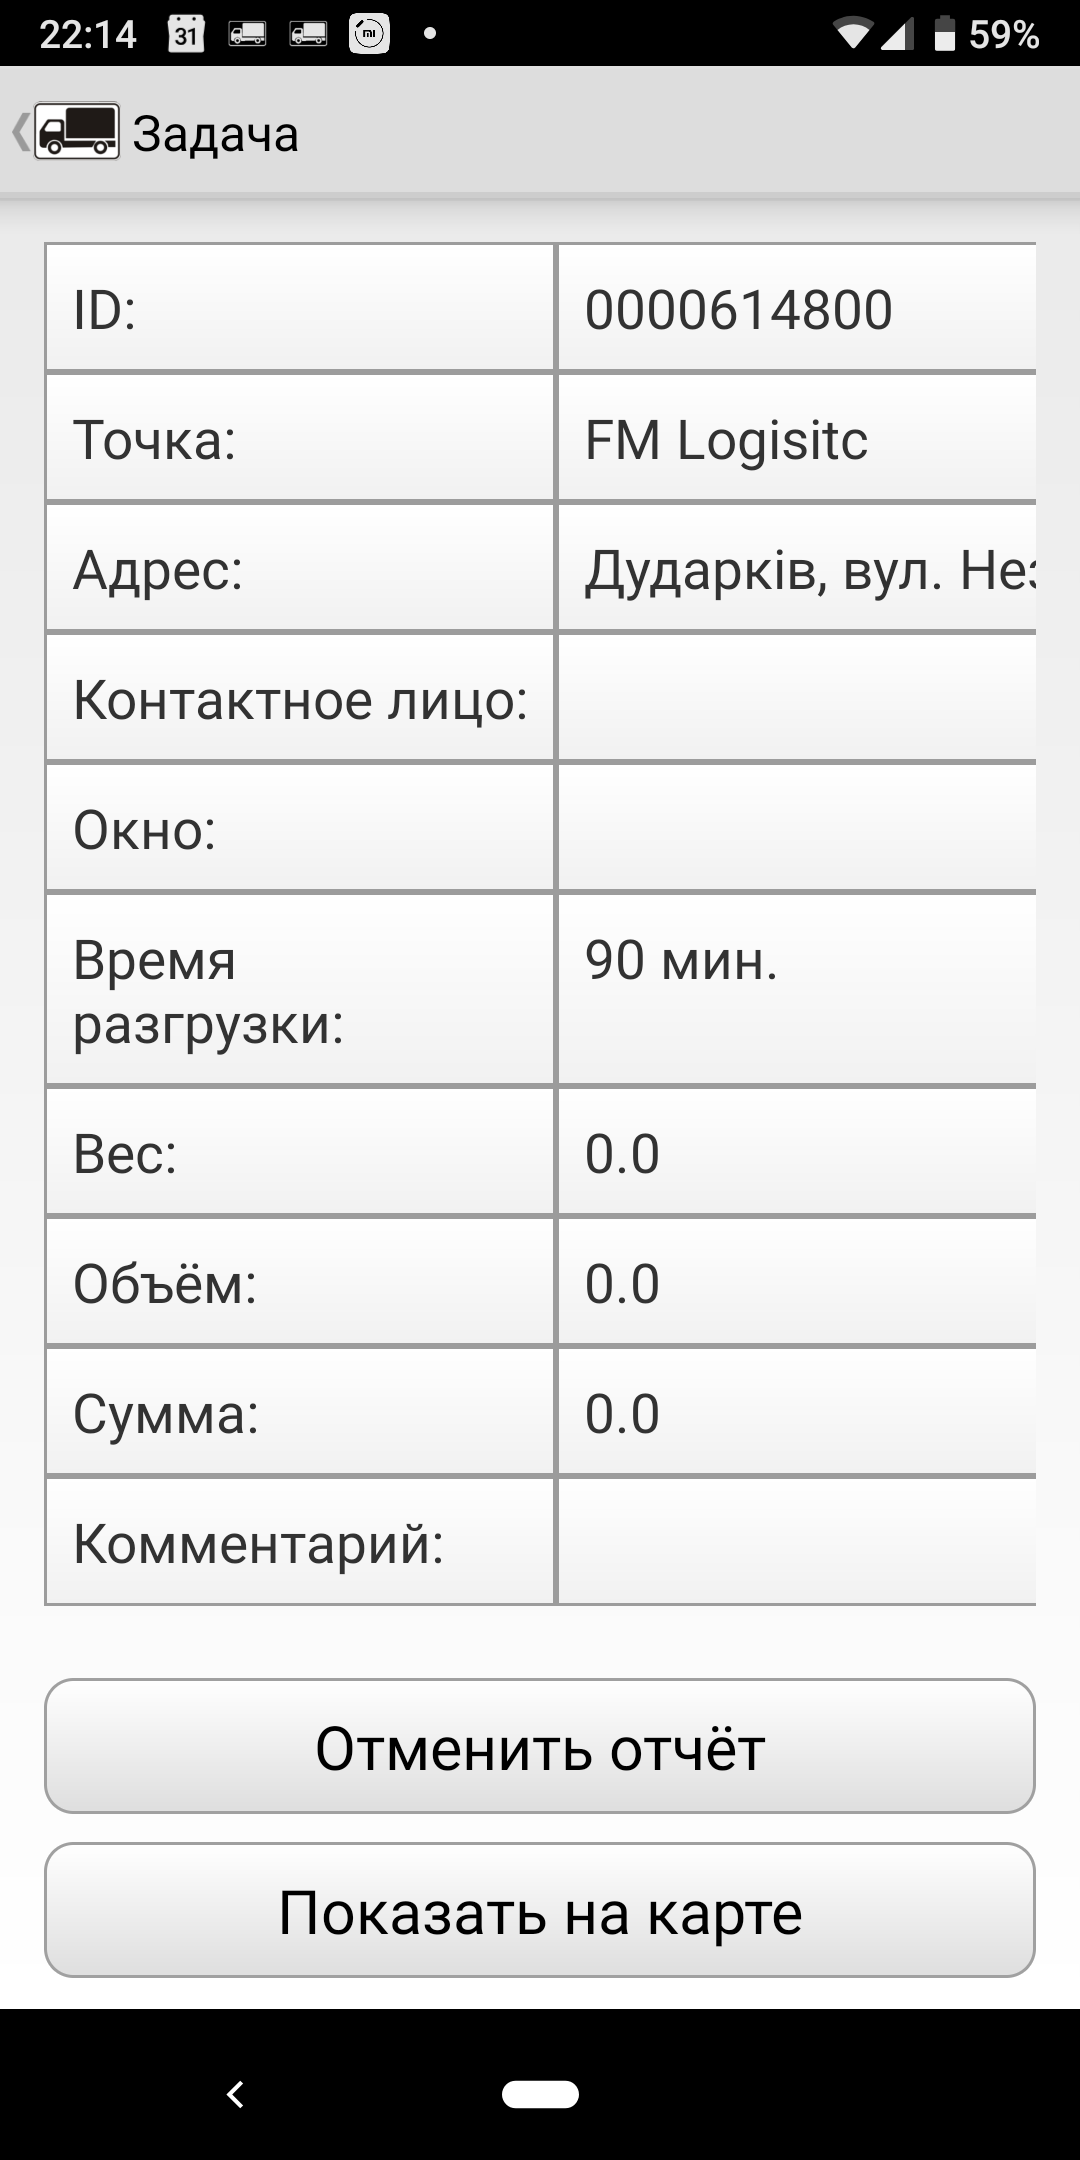
\includegraphics[width=.32\linewidth]{app-point}}
	\hspace{0pt plus2fill}
	\subbottom[\label{img:app-map}]{%
		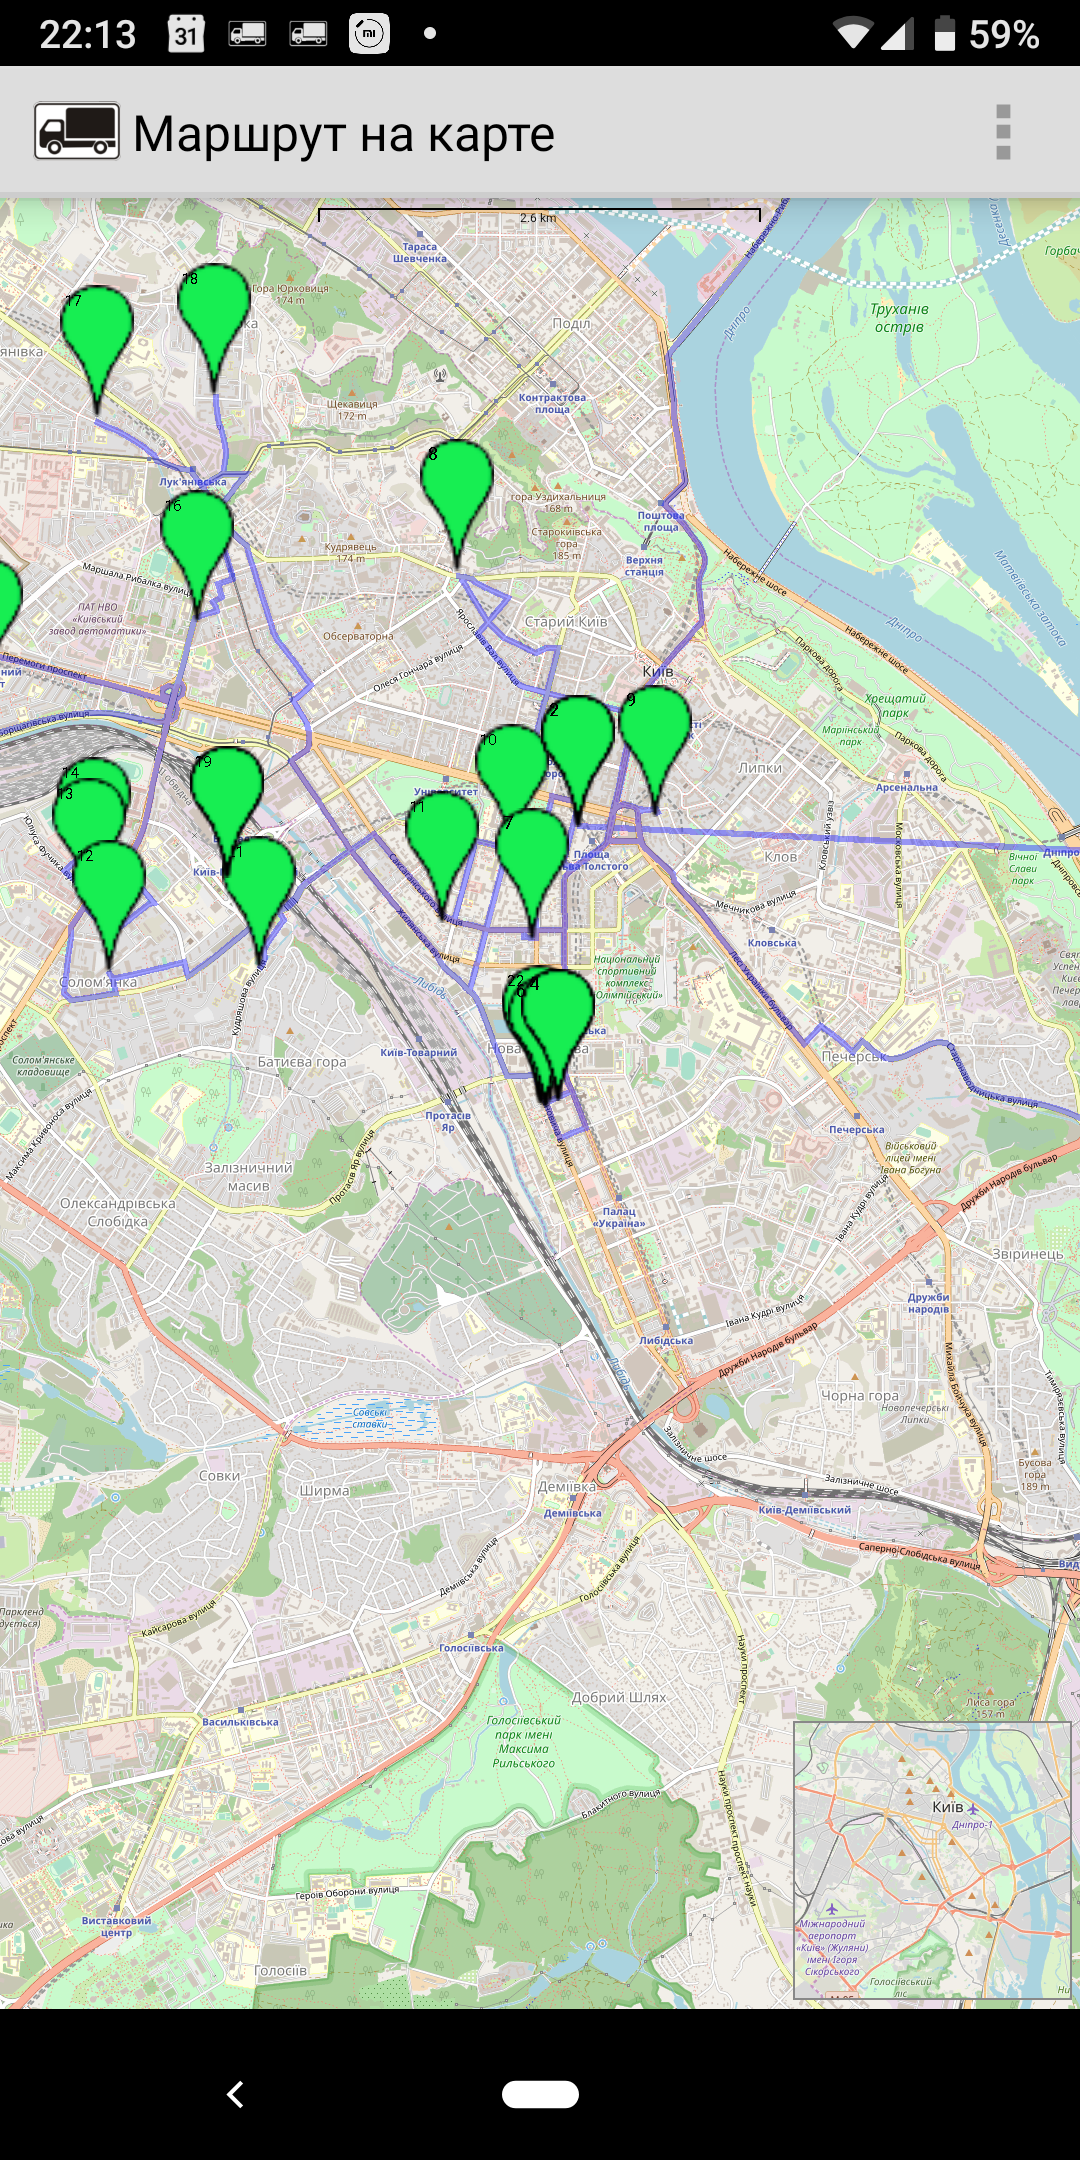
\includegraphics[width=.32\linewidth]{app-map}}
	\hspace{0pt plus2fill}
	\subbottom[\label{img:app-map-late}]{%
		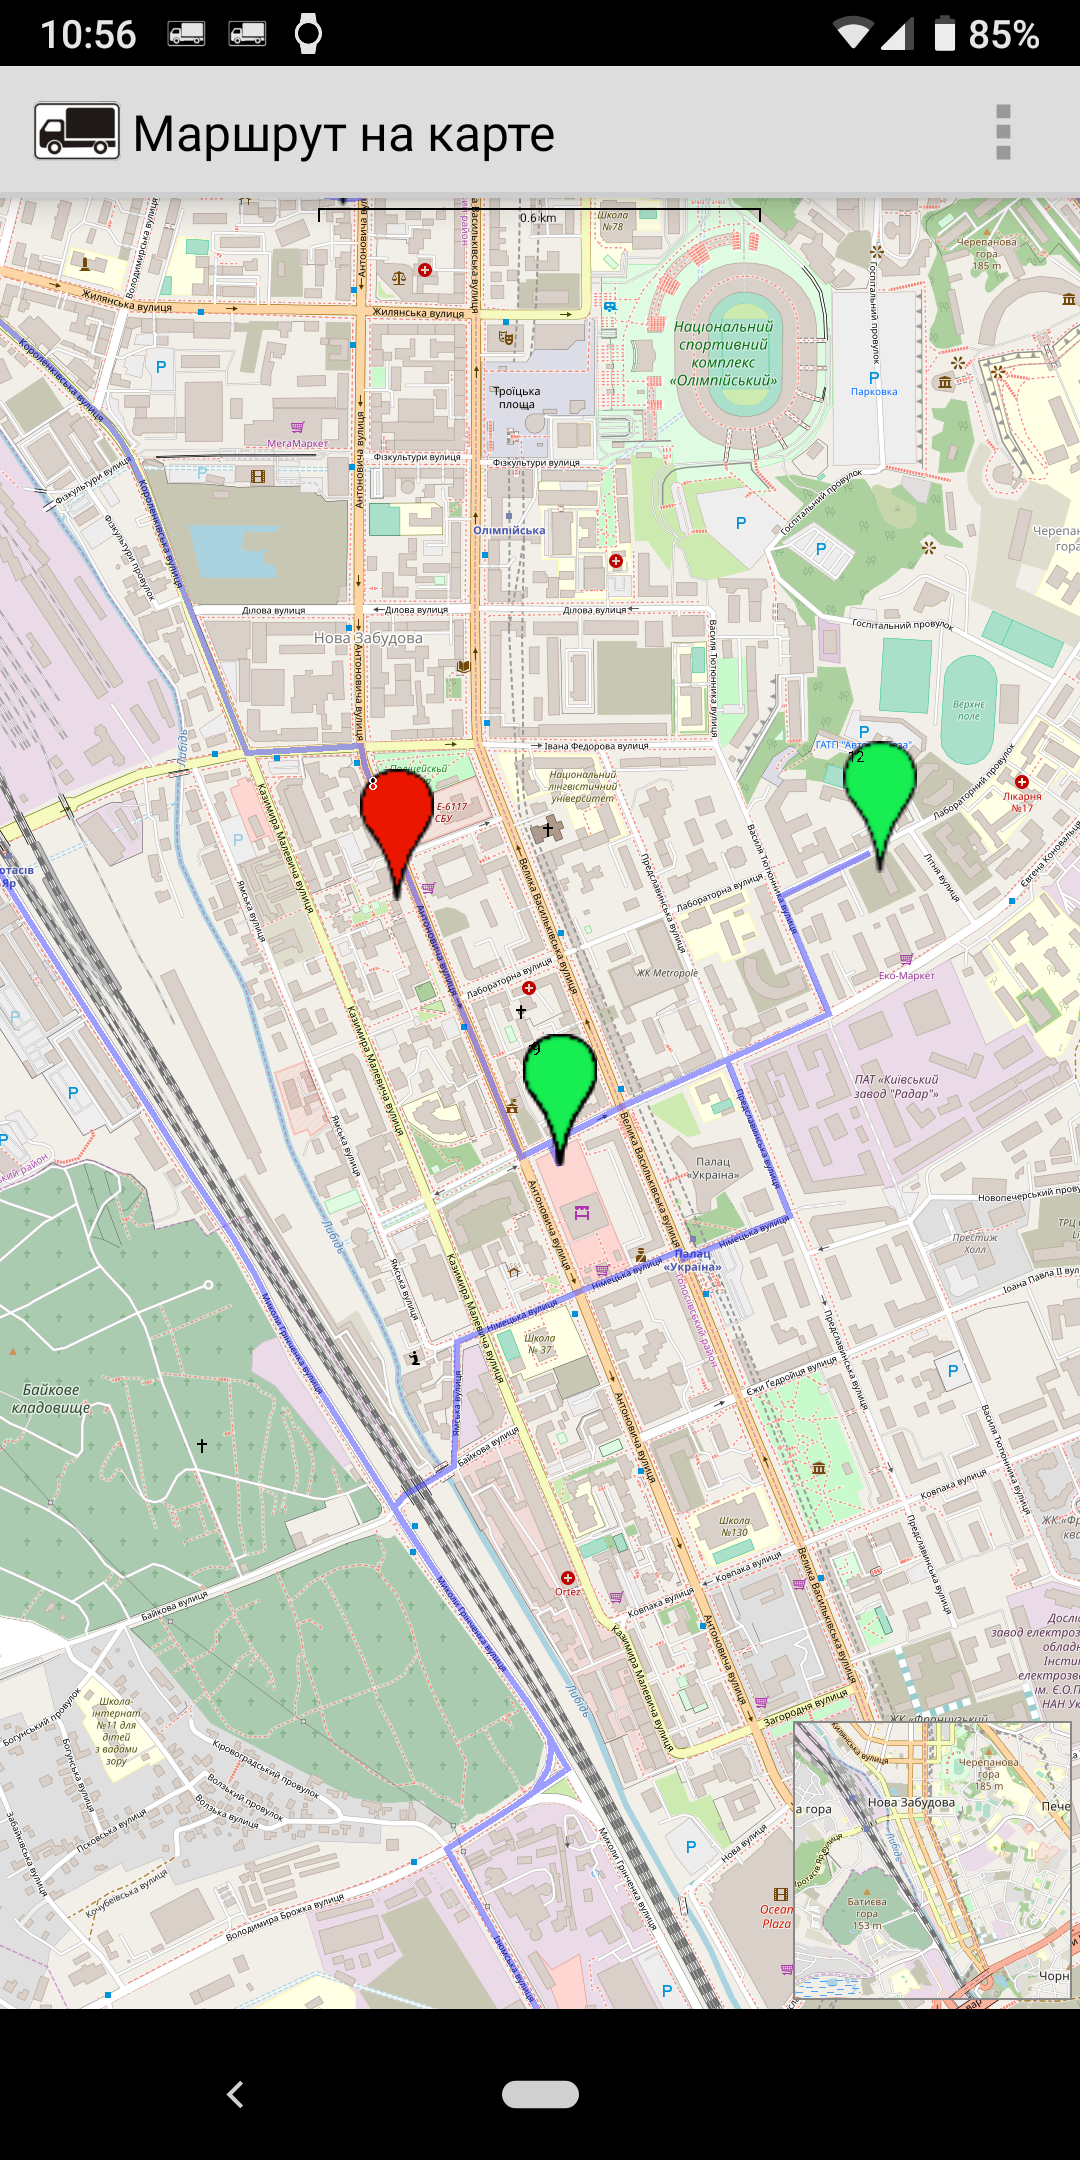
\includegraphics[width=.32\linewidth]{app-map-late}}
	\hspace{0pt plus1fill}
	\caption{Інтерфейс інформації про точку (\subcaptionref{img:app-point}) та мапи маршруту (\subcaptionref{img:app-map}), в тому числі з відміткою не виконаних точок (\subcaptionref{img:app-map-late})}
	\label{img:app-point-map}
\end{figure}

Для успішного використання додатку його треба зареєструвати в системі. Вигляд інтерфейсу для незареєстрованого пристрою зображена на рис. \ref{img:app-no1}. Самостійна реєстрація водієм неможлива, реєстрацію додатку та пристрою в системі диспетчерського контролю за рухом автотранспорту повинен провести адміністратор системи. Після реєстрації необхідно ввести логін та пароль у вікні налаштувань (рис. \ref{img:app-opt}). У випадку успішної реєстрації додаток перейде в інтерфейс загальної інформації про маршрут (рис. \ref{img:app-info}), або, якщо маршруту на вибрану дату не існує, повідомить про це (рис. \ref{img:app-no2}).

Крім введення логіну та паролю для реєстрації в системі, адміністратор також може встановити пароль адміністратора, щоб унеможливити доступ водія до налаштувань додатку. Основне призначення цієї функції, не дати водію втручатися в роботу важливих компонентів системи, таких як, наприклад, збір GPS даних. 

Вигляд інтерфейсу загальної інформації про маршрут зображено на рис. \ref{img:app-info}. У цьому вікні показана така інформація як імʼя водія-експедитора, модель та номер транспортного засобу, дата на яку складено маршрут доставки, тощо. Також у цьому вікні вказані поточні та підсумкові кількості точнок доставки за різними категоріями, такими як: загальна кількість точок у маршруті, кількість заїздів на склад, поточна кількість успішно та неуспішно виконаних точок, кількість точок яку ще необхідно буде виконати та прогнозні значення скільки з них водій встигає виконати вчасно, а в яку кількість він запізнюється (за нормальних транспортних умов).

Вікно маршрутного листа зображено на рис. \ref{img:app-list}. Цей інтерфейс містить таблицю точок доставки у необхідному порядку їх виконання. Таблиця містить таку інформацію про точки як: назву точки або імʼя контактної особи, адресу, запланований час прибуття та прогнозний час обслуговування точки. Рядки таблиці виділяются різним кольором в залежності від різного статусу точки, такі як: склад, точка виконана успішно, точка відмічена як не виконана або відмінена, точка запланована до виконання і прогноз прибуття до неї справджується або ж точка запланована до виконання, але прогноз показує ризик запізнення у точку.

При натисканні на будь-яку точку доставки, або при наданні відповідної голосової команди, буде показано вікно інформації про точку (рис. \ref{img:app-point}). Цей інтерфейс містить наступну інформацію про точку доставки: ідентифікаційний номер, назва точки доставки та імʼя контактної особи, адреса точки, часове вікно у яке дозволено виконувати доставку у точці (наприклад у випадку доставки товарів фізичній особі до початку робочого дня, це може бути з 7:00 до 9:00) та прогнозований час розвантаження. Крім того в інтерфейсі показані дані про вагу, обʼєм та вартість товару, що доставляється, а також будь-які коментарі клієнта чи диспетчера, щодо цієї точки.

Вигляд інтерфейсу мапи маршруту зображений на рис. \ref{img:app-map} та \ref{img:app-map-late}. Це вікно представляє собою карту, на якій різним кольором зображені точки доставки та можливий маршрут проїзду між ними. Колір точки залежить від статусу її доставки, та співпадає з кольором у таблиці маршрутного листа. Для навігації до точки може бути використаний сторонній додаток, такий як Google Maps, Яндекс карти чи інші. Вибрати додаток для навігації можна у вікні налаштувань (рис. \ref{img:app-opt}). При поступанні відповідної голосової команди, навігація автоматично почнеться за адресою вказаною у інформації про точку, а по прибутті на точку призначення інтерфейс повернеться до попереднього вікна.

Як можна бачити з скріншотів інтерфейсу мобільного додатку, більшість вікон мають інформаційних характер і призначені для того, щоб показувати додаткову інформацію при голосовому управлінні системою. Тим не менше основні функції переходу між вікнами програми та навігації продубльовані у вигляді сенсорних кнопок, що дозволяє отримати більш відмовостійкий інтерфейс.

Розроблений засіб формалізації голосової інформації дозволяє водію не відволікатись від управління автомобілем і слідкувати за дорожніми умовами та обстановкою, що дає змогу прискорити доставку продукції в процесі дистрибуції, а також підвищити рівень безпеки.

\section{Особливості використання засобів формалізації голосової інформації в системах диспетчерського контролю за рухом автотранспорту} \label{sect4_1}

Для водія автомобілю, який буде здійснювати доставку продукції в процесі дистрибуції і вперше зіштовхнеться з засобом формалізації голосової інформації, що діє в рамках системи диспетчерського контролю за рухом автотранспорту, буде включений навчальний курс роботи з даною системою, в ході якого йому буде необхідно навчити дану систему розпізнавати його особистий голос з відповідними конкретними словами чи командами. Використання таких засобів формалізації голосової інформації на борту автомобіля дозволяє розширити швидкодію водія в процесі дистрибуції, забезпечити і підвищити рівень безпеки.

У сучасних мобільних пристроях, таких, як смартфони Android та Iphone, уже існує функція розпізнавання голосу, але вона ще не може бути використана для задачі формалізації голосової інформації тому що:

\begin{itemize}
	\item Майже завжди ця функція для своєї роботи потребує постійного доступу до мережі інтернет. Оффлайн режим існує лише для деяких мов і має гіршу якість розпізнавання за рахунок обмеженого словника. Оскільки засіб розроблюється для водіїв, які можуть виконувати доставку в тому числі в віддалені місця --- навіть мобільного інтернет може бути не доступний, або швидкість передачі даних може бути занизька для роботи зі звуком.
	\item Класичні методи розпізнавання голосу дають на виході лексичний текст, який все одно треба аналізувати певними інтелектуальними системами, щоб визначити яка команда була сказана.
	\item В подальшому мережа покриття мобільного Інтернету буде розвиватися, тому використання вбудованих методів розпізнання голосу стане більш реалістичним. У такому випадку одним з потенційних варіантів розвитку розроблених засобів формалізації голосової інформації є їх модифікація для використання вбудованих методів розпізнання голосу у якості фонемного стенографа, і використовувати розпізнаний лексичний текст в запропонованій системі замість фонетичного, для розпізнавання команд вимовлених по різному.
\end{itemize}

Інтерактивний інтерфейс в системі формалізації голосової інформації дозволяє водієві розмовляти з автомобілем (технічним засобом), створювати запити, отримувати інформацію і вказівки, вирішувати завдання з доставки продукції, у рамках системи диспетчерського контролю за рухом автотранспорту.

Сама точність розпізнавання мови водія багато в чому визначається якістю і стабільністю його вимови. Тому для попереднього навчання водіїв в голосовому інтерфейсі даної системи формалізації голосової інформації з диспетчерським контролем за рухом автотранспорту застосовується інформаційна система навчання. Виникаюче в них завдання постановки вимови, становить інтерес через велику сферу практичного застосування в різних областях. При цьому виникає проблема варіативності усного мовлення водіїв для різних носіїв національної мови і тісно повʼязана з нею проблема самостійної оцінки якості своєї вимови. У наявності очевидне протиріччя в самій постановці завдання: той, якого навчають з недостатньою на даний момент мовною підготовкою та обмеженими можливостями в процесі самонавчання повинен наблизитися за своєю вимовою до деякого еталону, який він слабо собі уявляє. Зазначене протиріччя з успіхом долається в запропонованій системі формалізації голосової інформації з диспетчерським контролем за рухом автотранспорту на основі критерію мінімуму інформаційного неузгодженості – на основі фонем. У цьому підході досяжність еталонної вимови забезпечується використанням не одного, а декількох «еталонів», які включають в себе і кращі зразки вимовлянь від одного або, навіть, декількох водіїв, які успішно пройшли навчання раніше. Така система формалізації голосової інформації здатна запамʼятовувати кращі вимови водієм слів і оцінювати якість подальшого виголошення тих же слів по відношенню до цих найкращих для водія словам, а не тільки по відношенню до використовуваних за замовчуванням стандартам, введених ідеальним водієм (диктором). При цьому у системі формалізації голосової інформації з диспетчерським контролем за рухом автотранспорту для оцінки якості вимови використовується тестування розрізнення різних звуків, яке може бути здійснено за допомогою одного з відомих методів автоматичного розпізнавання мови – пофонемного. У попередньому розділі показано, що для підвищення точності розпізнавання мови водія можуть бути застосовані ЗНМ.

При розробці систем розпізнавання дуже важливу роль грає експериментальний матеріал, на якому перевіряються і досліджуються запропоновані ідеї. В області розпізнавання мови в розробленій системі формалізації голосової інформації з диспетчерським контролем за рухом автотранспорту цей матеріал (слова і команди) є еталоном, який знаходиться в проміжній базі даних. По-іншому, таку базу даних можна позначити як корпус. Хоча корпуси усного мовлення вперше стали створювати для проведення фонетичних досліджень мови, широка потреба в них виникла, в значній мірі, завдяки розробкам в області автоматичного розпізнавання мови. На жаль, не існує універсальних мовних баз, які підійшли б для будь-якого завдання в області розпізнавання мови або фонетичних досліджень. Структура і склад мовного корпусу визначаються завданнями, які ставляться перед системою розпізнавання, яка використовує цей корпус.

У базі даних еталонів мовних фонем для систем голосового управління зібрано значну кількість необхідних прикладів виголошення заявлених для розпізнавання команд засобом формалізації голосової інформації в системах диспетчерського контролю за рухом автотранспорту.

Під час створення бази даних еталонів мовних фонем необхідно було вирішити чотири групи питань: технічні, змістовні, структурні та інструментальні (виконавчі).

Технічні питання повʼязані з вибором програмно-апаратних засобів запису мовного матеріалу (еталонів), а також з організацією необхідних умов запису, наприклад, виключення фонового шуму у засобах формалізації голосової інформації в системах диспетчерського контролю за рухом автотранспорту.

Змістовні питання в системі формалізації голосової інформації з диспетчерським контролем за рухом автотранспорту стосуються складу бази даних, а саме:

\begin{itemize}
	\item з вибором водіїв (дикторів) (кількість, стать, вік, діалектні відмінності тощо);
	\item з підбором текстового матеріалу (спеціалізований / репрезентативний, тип вимовлених мовних зразків (слова, команди, окремі пропозиції, тексти, зразки спонтанного мовлення), фонетично збалансований / незбалансований, тип балансування, статистичне представництво звукових одиниць тощо);
	\item з розподілом текстового матеріалу за водіями (дикторами), включаючи кількість підходів для кожного з них;
	\item з розподілом мовного матеріалу серед водіїв на тренувальну і тестову частини;
	\item з вибором типів інформації, яка асоціюється з кожним звуковим файлом (орфографічний запис, фонемний запис / фонетична транскрипція реального виголошення, акустико-фонетична розмітка звукового сигналу, інші типи анотацій і коментарів).
\end{itemize}

Структурні питання в системі формалізації голосової інформації з диспетчерським контролем за рухом автотранспорту визначають спосіб організації інформації, що міститься в базі даних еталонів, що повʼязані зі структурою директорій і файлів, зі створенням протоколів тощо.

До інструментальних питань в системі формалізації голосової інформації відносяться питання, що виникають у звʼязку з автоматизацією і стандартизацією різних етапів створення бази даних еталонів мовних фонем. При цьому в системі формалізації голосової інформації з диспетчерським контролем за рухом автотранспорту передбачені інструменти, що полегшують процеси транскрибування і структурування записаного матеріалу. Для цього у системі формалізації голосової інформації створена спеціальна програма, яка працює за методом суфлера (prompt-method). Дана програма дозволяє безпосередньо в процесі запису створювати звукові файли, що відповідають окремим обʼєктам бази даних еталонів мовних фонем.

Як було зазначено вище, структуру і склад мовної бази системи формалізації голосової інформації з диспетчерським контролем за рухом автотранспорту визначають коло завдань, що вирішуються розробленою системою розпізнавання голосу.

У даній роботі при розробці засобів формалізації голосової інформації в системах диспетчерського контролю за рухом автотранспорту стояло завдання дослідити запропоновані методи розпізнавання слів (фонем) і їх реалізації в системі формалізації голосової інформації. Це дослідження можна провести на вирішенні задачі розпізнавання голосових команд. При такій спеціалізації програмного комплексу системи формалізації голосової інформації з диспетчерським контролем за рухом автотранспорту досягаються дві мети. По-перше, засіб розпізнавання голосових команд – центральний компонент системи формалізації голосової інформації, актуальність розробки якої позначена на початку даної роботи. По-друге, розширення завдання до розпізнавання злитого і спонтанного мовлення призвело б до невиправданого ускладнення програмного комплексу, викликаного необхідністю інтеграції СММ з лінгвістичної і іншими моделями мови.

Для проведення досліджень в рамках виконання дисертаційної роботи була складена власна база даних еталонів. Це було необхідно з наступних причин. По-перше, внаслідок специфіки розробляємої системи формалізації голосової інформації з диспетчерським контролем за рухом автотранспорту і завдань, які вона вирішує, знайти ідеально підходящу за структурою і складом базу даних еталонів мовних фонем неможливо; найбільш поширені бази даних (корпуси) з високою варіативністю звуків мови, що підійшло б для навчання і тестування систем розпізнавання спонтанної мови. По-друге, безкоштовних баз даних еталонів мовних фонем (корпусів) просто не існує. Нарешті, для наочності та усунення можливих лінгвістичних складнощів, найкращий був би корпус української або російської мови.

Склад створеної бази даних еталонів мовних фонем відповідає завданням, покладеним на систему формалізації голосової інформації з диспетчерським контролем за рухом автотранспорту. По-перше, кількість класів відповідає можливому числу і складу команд для розробленої системи голосового управління, включаючи числівники («один», «два», «перший», «другий» тощо), наприклад, для набору координат, і покажчики напрямку («прямо», «вправо», «вперед» тощо). По-друге, важливою рисою складеної бази даних еталонів мовних фонем є те, що усі навчальні і тестові приклади не перетинаються, що істотно підвищує достовірність результатів експериментальної перевірки системи формалізації голосової інформації. Процес побудови бази даних еталонів системи формалізації голосової інформації був автоматизований за допомогою розроблених програмних засобів попередньої обробки і поділу необхідних прикладів виголошення команд на окремі файли. Для обʼєднання окремих етапів була використана скриптова мова та деякі засоби автоматизації \cite{tange_ole_2018_1146014}.

В ідеалі результатом розпізнавання фонем, що утворюють слово, як зазначалось, є його транскрипція, за якою слово в більшості випадків однозначно відновлюється. Однак, будь-які ознаки, що використовуються при розпізнаванні мови, мають характер випадкових величин. Тому на будь-якому етапі можлива відмова від розпізнавання і в результаті замість ланцюжка транскрипційних знаків на виході вийде послідовність символів, що позначають ті чи інші досить широкі класи фонем. Їх можна розглядати як результат змішання транскрипцій різного рівня деталізації. Виникає проблема, повʼязана з тим: як за таким різнорідним результатом у словнику команд (базі управління) відшукати необхідні слова, які йому задовольняють. 

У системі формалізації голосової інформації з диспетчерським контролем за рухом автотранспорту застосовано алгоритм, який дозволяє зробити це дуже швидко. Виграш в продуктивності став можливий завдяки структурі дерева сценаріїв, яке запропоновано в третьому розділі. Більш того, такий підхід виявляється корисним і в разі пошуку слів за узагальненою транскрипцією. Обхід дерева сценаріїв з підстановкою різних варіантів написання слова (фонеми) за узагальненою транскрипцією на кожному рівні дерева (тобто генерація варіантів написання слова за узагальненою транскрипцією в контексті вихідного словника команд для порівняння з навчальною вибіркою) скорочує значення M на кілька порядків.
Тобто кожен рівень дерева сценаріїв відповідає позиції контексту, що присутній у словнику команд (базі управління). Кожен вузол в рамках кожного рівня дерева є символ в слові відповідного контексту.

Для системи формалізації голосової інформації з диспетчерським контролем за рухом автотранспорту був розроблений засіб (додаток на мобільному пристрої) для збору голосових даних водіїв, експериментальні дані для якого наведені нижче.

\section{Апробація засобів формалізації голосової інформації в системах диспетчерського контролю за рухом автотранспорту} \label{sect4_2}

З метою перевірки ефективності побудованих моделей було проведено ітеративний процес збору даних та моделювання, який передбачав аналіз отриманих результатів та введення нових критеріїв оцінки, якщо попередні не давали достатньої точності оцінювання. У цілому цей процес апробації засобів формалізації голосової інформації в системах диспетчерського контролю за рухом автотранспорту можна розбити на три основні етапи.

На першому етапі була зібрана широка вибірка голосових даних згідно із моделлю дерева сценаріїв голосової взаємодії в системах підтримки диспетчеризації автотранспорту. Зібрані голосові дані можна охарактеризувати наступними параметрами:

\begin{itemize}
	\item 4 пристрої, 23 диктори (11 жінок, 12 чоловіків), 94 варіанти стимулів (64 на основні реакції), 3046 зразків;
	\item додатково 23 варіанти стимулів та 465 голосових зразків для реакції розпізнавання часу.
\end{itemize}

Детальний розподіл голосових даних, зібраних на першому етапі моделювання, представлено в таблиці \ref{tbl:data1_distribution}. Ця таблиця показує розподіл зібраних голосових зразків за пристроями та дикторами, а також повідомляє загальну кількість голосових зразків надиктованих кожним диктором, кількість унікальних реакцій та варіантів формулювання стимулів різними словами серед зібраних голосових зразків. В окрему колонку виведено кількість додаткових записів для реакції розпізнавання часу.

\begin{mytable}[ht]{ | c | c | c | c | c | c | c | }%
	{Детальний розподіл за дикторами та пристроями голосових даних зібраних на першому етапі моделювання}%
	{\label{tbl:data1_distribution}}%
	{
		\specialcell{3cm}{Диктор} & 
		\specialcell{3cm}{Пристрій} & 
		\specialcell{3cm}{Стать} & 
		\specialcell{3cm}{Кількість \\ записів} & 
		\specialcell{3cm}{Кількість \\ реакцій} &
		\specialcell{3cm}{Кількість \\ варіантів \\ стимулів} & 
		\specialcell{3cm}{Кількість \\ записів \\ реакції часу}}
	
	1 & 1 & жін. & 109 & 64 & 92 & 22 \\
	\hline
	2 & 1 & жін. & 105 & 64 & 96 & 22 \\
	\hline
	3 & 1 & жін. & 100 & 64 & 96 & 21 \\
	\hline
	4 & 1 & жін. & 97 & 64 & 93 & 22 \\
	\hline
	5 & 1 & жін. & 96 & 64 & 93 & 22 \\
	\hline
	6 & 1 & жін. & 95 & 64 & 94 & 22 \\
	\hline
	7 & 1 & жін. & 95 & 64 & 95 & 23 \\
	\hline
	8 & 1 & жін. & 95 & 62 & 90 & 21 \\
	\hline
	9 & 1 & жін. & 90 & 62 & 89 & 22 \\
	\hline
	10 & 1 & жін. & 79 & 58 & 79 & 23 \\
	\hline
	11 & 1 & чол. & 196 & 64 & 96 & 44 \\
	\hline
	12 & 1 & чол. & 101 & 64 & 94 & 25 \\
	\hline
	13 & 1 & чол. & 96 & 64 & 92 & 22 \\
	\hline
	14 & 1 & чол. & 98 & 63 & 95 & 21 \\
	\hline
	15 & 1 & чол. & 89 & 63 & 85 & 22 \\
	\hline
	16 & 1 & чол. & 98 & 62 & 90 & 21 \\
	\hline
	17 & 1 & чол. & 64 & 48 & 62 & 22 \\
	\hline
	18 & 1 & чол. & 30 & 25 & 30 & 0 \\
	\hline
	19 & 1 & чол. & 23 & 16 & 22 & 0 \\
	\hline
	20 & 1 & чол. & 23 & 9 & 19 & 0 \\
	\hline
	21 & 2 & жін. & 97 & 64 & 94 & 22 \\
	\hline
	22 & 3 & чол. & 96 & 64 & 96 & 22 \\
	\hline
	23 & 4 & чол. & 99 & 64 & 96 & 24 \\
	
\end{mytable}

Як можна бачити, не всі диктори надиктували повний перелік реакцій згідно до моделі голосової взаємодії в системах підтримки диспетчеризації. Це має сенс, оскільки не всі водії будуть стикатися з усіма можливими позаплановими подіями. Також деякі диктори надиктували повністю ідентичні фрази кілька разів, що б мати можливість виключити вплив сторонніх шумів і певної стохастичності вимови та запису звуку, а деякі диктори надиктували різні варіанти формулювання та вимови стимулів, що б мати можливість навчити систему виділяти ключову інформацію в різних формулюваннях природної мови.

Першим було проведене моделювання методом інтелектуальних рефлекторних систем з розміром N-грам 1–3. Результати моделювання наведено в таблиці \ref{tbl:total_data1_irs13}. Було створено окрему модель для кожного контексту взаємодії водія та системи підтримки диспетчеризації автотранспорту, а також модель розпізнавання реакцій для всієї вибірки, без використання контекстів. Крім контекстів, представлених у моделі голосової взаємодії, було використано додатковий тестовий контекст, який складався з трьох реакцій найпростішого дерева сценаріїв голосової взаємодії \cite{art3}.

\begin{mytable}[ht]{ | c | c | c | c | c | c | }%
	{Результати моделювання першого набору даних використовуючи ІРС з послідовностями розміром 1--3}%
	{\label{tbl:total_data1_irs13}}%
	{
		\specialcell{3cm}{№ Контексту} & 
		\specialcell{3cm}{Точність \\ розпізнання} & 
		\specialcell{3cm}{Середня \\ прецизійність} & 
		\specialcell{3cm}{Середня \\ повнота} & 
		\specialcell{3cm}{Середня \\ F-міра} & 
		\specialcell{3cm}{Кількість}}	
	
	1 & 0.677 & 0.450 & 0.445 & 0.447 & 124 \\
\hline
2 & 0.456 & 0.559 & 0.663 & 0.408 & 513 \\
\hline
3 & 0.387 & 0.055 & 0.143 & 0.080 & 217 \\
\hline
4 & 0.375 & 0.217 & 0.271 & 0.171 & 104 \\
\hline
5 & 0.339 & 0.108 & 0.184 & 0.111 & 183 \\
\hline
6 & 0.397 & 0.198 & 0.252 & 0.222 & 209 \\
\hline
7 & 0.206 & 0.021 & 0.098 & 0.034 & 233 \\
\hline
8 & 0.346 & 0.182 & 0.179 & 0.107 & 217 \\
\hline
9 & 0.344 & 0.144 & 0.225 & 0.141 & 131 \\
\hline
10 & 0.349 & 0.489 & 0.255 & 0.194 & 126 \\
\hline
11 & 0.268 & 0.099 & 0.145 & 0.114 & 239 \\
\hline
12 & 0.264 & 0.303 & 0.250 & 0.238 & 201 \\
\hline
13 & 0.450 & 0.361 & 0.259 & 0.182 & 171 \\
\hline
14 & 0.439 & 0.551 & 0.432 & 0.432 & 139 \\
\hline
15 & 0.302 & 0.547 & 0.210 & 0.152 & 159 \\
\hline
16 & 0.478 & 0.539 & 0.470 & 0.450 & 115 \\
\hline
17 & 0.271 & 0.261 & 0.263 & 0.248 & 155 \\
\hline
18 & 0.418 & 0.482 & 0.411 & 0.407 & 110 \\
\hline
19 & 0.471 & 0.650 & 0.458 & 0.462 & 87 \\
\hline
\specialcell{3cm}{По всій \\ вибірці} & 0.044 & 0.027 & 0.017 & 0.009 & 2069 \\
\hline
\specialcell{3cm}{Тестовий \\ контекст} & 0.485 & 0.162 & 0.333 & 0.218 & 101 \\
\end{mytable}

Розміри N-грам 1–3 було обрано, виходячи з того, що метод інтелектуальних рефлекторних систем має квадратичну залежність швидкості розрахунку від максимального розміру N-грам. З таблиці \ref{tbl:total_data1_irs13}  видно, що точність розпізнавання цих моделей не перевищує 50\% для жодного з контекстів, крім першого. Тому для підвищення якості моделей було проведено моделювання цим же методом, але з розміром N-грам 2–4. Результати цього моделювання представлено в таблиці \ref{tbl:total_data1_irs24}.

\begin{mytable}[ht]{ | c | c | c | c | c | c | }%
	{Результати моделювання першого набору даних використовуючи ІРС з послідовностями розміром 2--4}%
	{\label{tbl:total_data1_irs24}}%
	{
		\specialcell{3cm}{№ Контексту} & 
		\specialcell{3cm}{Точність \\ розпізнання} & 
		\specialcell{3cm}{Середня \\ прецизійність} & 
		\specialcell{3cm}{Середня \\ повнота} & 
		\specialcell{3cm}{Середня \\ F-міра} & 
		\specialcell{3cm}{Кількість}}	
	
	1 & 0.710 & 0.503 & 0.442 & 0.459 & 124 \\
\hline
2 & 0.895 & 0.465 & 0.478 & 0.471 & 513 \\
\hline
3 & 0.382 & 0.048 & 0.124 & 0.069 & 217 \\
\hline
4 & 0.558 & 0.740 & 0.480 & 0.484 & 104 \\
\hline
5 & 0.415 & 0.434 & 0.259 & 0.225 & 183 \\
\hline
6 & 0.565 & 0.282 & 0.359 & 0.316 & 209 \\
\hline
7 & 0.232 & 0.388 & 0.127 & 0.089 & 233 \\
\hline
8 & 0.373 & 0.410 & 0.207 & 0.157 & 217 \\
\hline
9 & 0.527 & 0.737 & 0.437 & 0.449 & 131 \\
\hline
10 & 0.532 & 0.773 & 0.468 & 0.486 & 126 \\
\hline
11 & 0.515 & 0.207 & 0.282 & 0.238 & 239 \\
\hline
12 & 0.488 & 0.510 & 0.469 & 0.452 & 201 \\
\hline
13 & 0.485 & 0.448 & 0.303 & 0.283 & 171 \\
\hline
14 & 0.633 & 0.703 & 0.625 & 0.625 & 139 \\
\hline
15 & 0.453 & 0.480 & 0.329 & 0.333 & 159 \\
\hline
16 & 0.583 & 0.661 & 0.574 & 0.550 & 115 \\
\hline
17 & 0.387 & 0.473 & 0.378 & 0.374 & 155 \\
\hline
18 & 0.582 & 0.672 & 0.576 & 0.583 & 110 \\
\hline
19 & 0.655 & 0.728 & 0.650 & 0.642 & 87 \\
\hline
\specialcell{3cm}{По всій \\ вибірці} & 0.122 & 0.061 & 0.048 & 0.027 & 2069 \\
\hline
\specialcell{3cm}{Тестовий \\ контекст} & 0.475 & 0.160 & 0.327 & 0.215 & 101 \\
\end{mytable}

Як альтернативний класифікатор у дуальній системі класифікації фонемної репрезентації голосових команд використано метод згорткових нейронних мереж \cite{art4}. На відміну від методу інтелектуальних рефлекторних систем, метод згорткових нейронних мереж залежить від розміру фільтрів лише лінійно, оскільки замість всіх можливих наборів N-грам, використовується лише певна фіксована кількість фільтрів, які навчаються методом зворотного розповсюдження помилки. Тому для моделювання методом згорткових нейронних мереж використовувалися лише фільтри розміром 2–4. Результати цього моделювання представлено в таблиці \ref{tbl:total_data1_cnn}.

\begin{mytable}[ht]{ | c | c | c | c | c | c | }%
	{Результати моделювання першого набору даних використовуючи ЗНМ з послідовностями розміром 2--4}%
	{\label{tbl:total_data1_cnn}}%
	{
		\specialcell{3cm}{№ Контексту} & 
		\specialcell{3cm}{Точність \\ розпізнання} & 
		\specialcell{3cm}{Середня \\ прецизійність} & 
		\specialcell{3cm}{Середня \\ повнота} & 
		\specialcell{3cm}{Середня \\ F-міра} & 
		\specialcell{3cm}{Кількість}}	
	
	1 & 0.879 & 0.880 & 0.863 & 0.870 & 124 \\
\hline
2 & 0.957 & 0.933 & 0.799 & 0.851 & 513 \\
\hline
3 & 0.820 & 0.870 & 0.777 & 0.813 & 217 \\
\hline
4 & 0.846 & 0.857 & 0.829 & 0.837 & 104 \\
\hline
5 & 0.798 & 0.814 & 0.734 & 0.754 & 183 \\
\hline
6 & 0.852 & 0.851 & 0.789 & 0.814 & 209 \\
\hline
7 & 0.785 & 0.808 & 0.773 & 0.785 & 233 \\
\hline
8 & 0.871 & 0.895 & 0.847 & 0.867 & 217 \\
\hline
9 & 0.863 & 0.871 & 0.836 & 0.847 & 131 \\
\hline
10 & 0.825 & 0.841 & 0.818 & 0.819 & 126 \\
\hline
11 & 0.908 & 0.922 & 0.850 & 0.878 & 239 \\
\hline
12 & 0.846 & 0.852 & 0.849 & 0.847 & 201 \\
\hline
13 & 0.848 & 0.860 & 0.842 & 0.849 & 171 \\
\hline
14 & 0.842 & 0.851 & 0.838 & 0.838 & 139 \\
\hline
15 & 0.849 & 0.842 & 0.829 & 0.834 & 159 \\
\hline
16 & 0.817 & 0.826 & 0.814 & 0.814 & 115 \\
\hline
17 & 0.723 & 0.729 & 0.723 & 0.720 & 155 \\
\hline
18 & 0.836 & 0.842 & 0.837 & 0.835 & 110 \\
\hline
19 & 0.862 & 0.871 & 0.863 & 0.856 & 87 \\
\hline
\specialcell{3cm}{По всій \\ вибірці} & 0.652 & 0.679 & 0.622 & 0.640 & 2069 \\
\hline
\specialcell{3cm}{Тестовий \\ контекст} & 0.891 & 0.915 & 0.871 & 0.888 & 101 \\
\end{mytable}

Таблиці \ref{tbl:total_data1_irs13}, \ref{tbl:total_data1_irs24} та \ref{tbl:total_data1_cnn} включають деякі міри оцінки якості моделей та кількість звукових записів, які використовувалися для навчання та оцінки моделей. Спочатку в якості основної міри використовувалася точність (accuracy) \cite{Ting_2011}, що може бути розрахована за наступною формулою:

\begin{equation}
\label{eq:acuracy}
A=\frac{\sum\limits_i TP_i}{\sum\limits_i TP_i+FN_i},
\end{equation}

де $A$ --- точність, $TP_i$ --- кількість вірно розпізнаних (True positive) зразків реакції $i$, a $FN_i$ --- кількість зразків реакції $i$, хибно розпізнаних (False negative) як інша реакція.

Оскільки частота реакцій у більшості контекстів не збалансована, точність може показувати кращі результати, ніж справжня якість моделі.

Побудувавши графіки розподілу точності та F-міри від кількості зразків у контексті (рис. \ref{img:accuracy_distribution_data1}) ми можемо бачити, що прямої залежності немає. Але на якість розпізнавання повинна впливати кількість реакцій в контексті і середня кількість записів зразків голосових даних на кожну реакцію.

\begin{figure}[!t]
	\centering
	\subbottom[Метод ІРС розміром 1--3 \label{img:accuracy_distribution_data1_irs13}]{%
		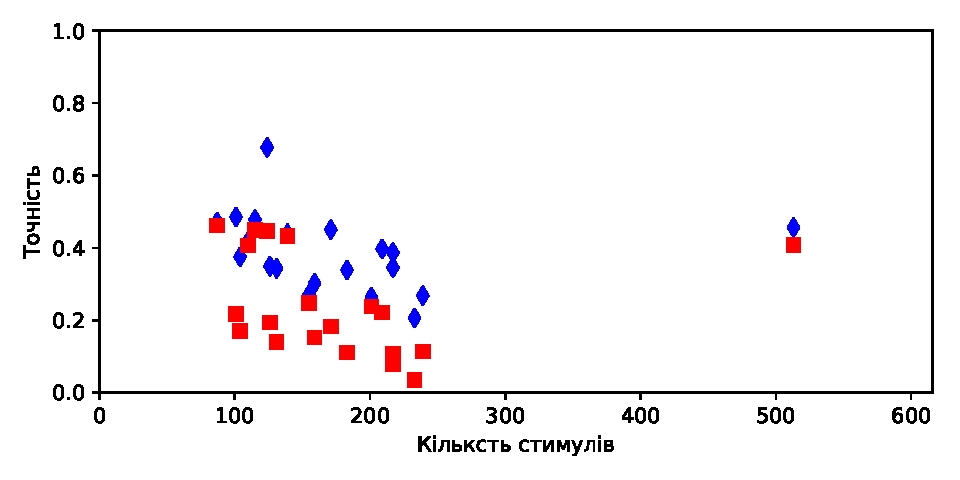
\includegraphics[width=.7\linewidth]{accuracy_distribution_data1_irs13}}
	\\
	\subbottom[Метод ІРС розміром 2--4 \label{img:accuracy_distribution_data1_irs24}]{%
		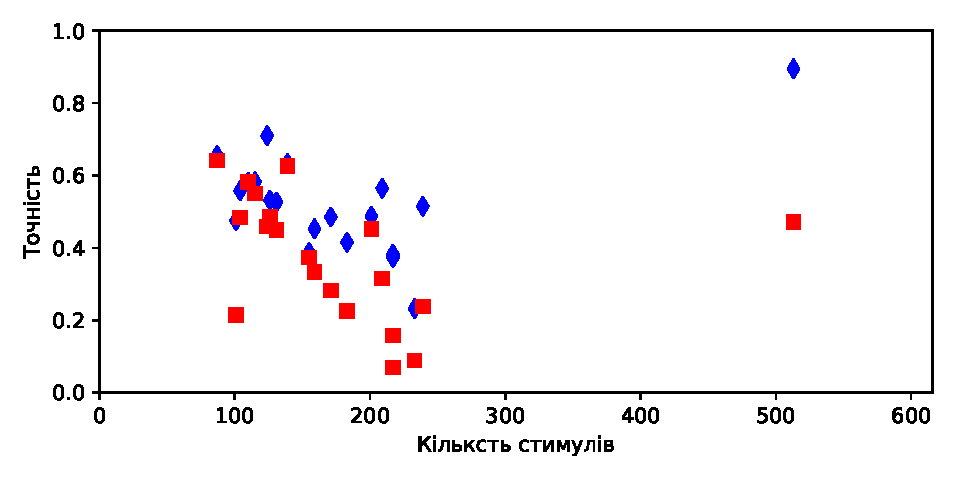
\includegraphics[width=.7\linewidth]{accuracy_distribution_data1_irs24}}
	\\
	\subbottom[Метод ЗНМ \label{img:accuracy_distribution_data1_cnn}]{%
		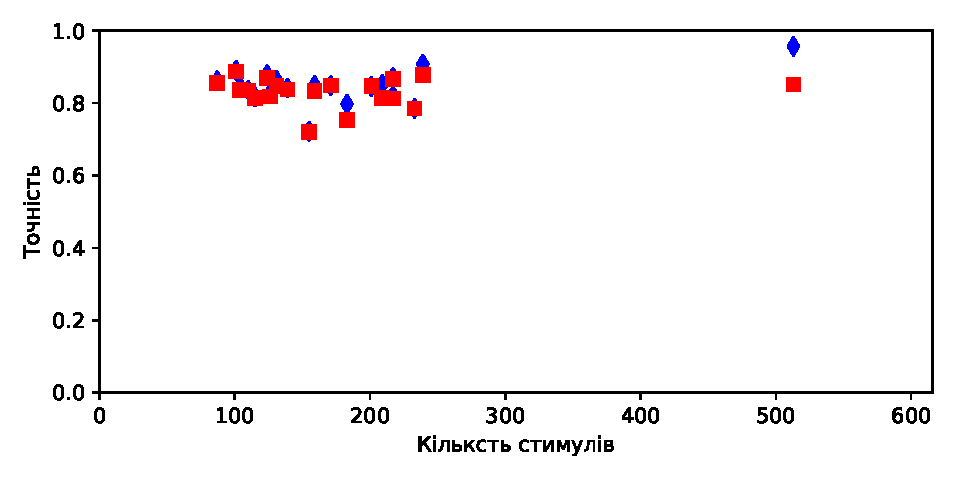
\includegraphics[width=.7\linewidth]{accuracy_distribution_data1_cnn}}
	\caption{Розподіл точності (червоні квадрати) та F-міри (сині ромби) за кількістю голосових зразків при моделюванні контекстів першого набору даних різними методами}
	\label{img:accuracy_distribution_data1}
\end{figure}

З матриці помилок (confusion matrix) \cite{Stehman_1997} моделювання тестового контексту методом інтелектуальних рефлекторних систем (рис. \ref{img:confusion_matrix_data1_irs13_context_21} та \ref{img:confusion_matrix_data1_irs24_context_21}), ми можемо бачити, що рівень розпізнавання близький до 50\% досягається за рахунок того, що всі реакції в контексті розпізнаються, як реакція №2. Оскільки вона представлена найбільшою кількістю зразків, точність досягає відносно високих значень при насправді низькій якості моделі.

\begin{figure}[!t]
	\centering
	\subbottom[Метод ІРС розміром 1--3 \label{img:confusion_matrix_data1_irs13_context_21}]{%
		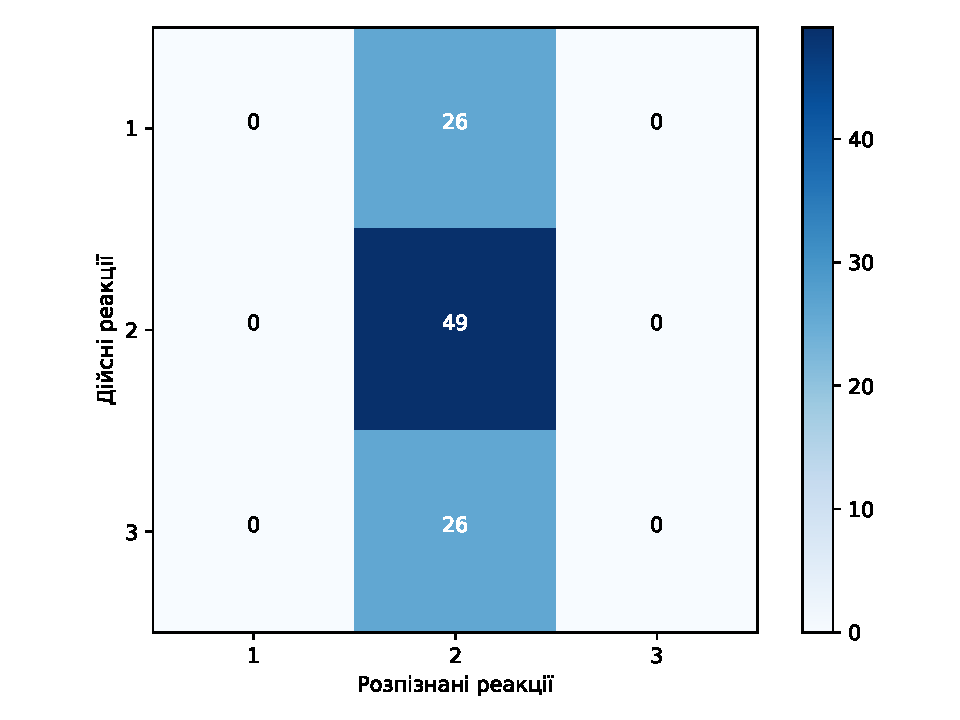
\includegraphics[width=0.3\linewidth]{confusion_matrix_data1_irs13_context_21}}
	\subbottom[Метод ІРС розміром 2--4 \label{img:confusion_matrix_data1_irs24_context_21}]{%
		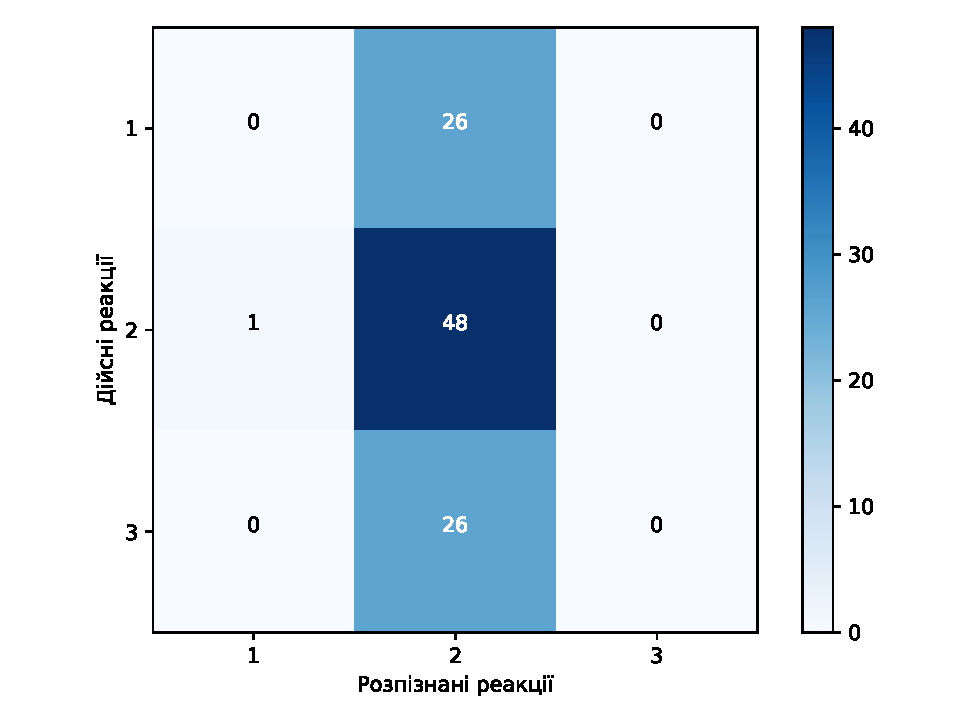
\includegraphics[width=0.3\linewidth]{confusion_matrix_data1_irs24_context_21}}
	\subbottom[Метод ЗНМ \label{img:confusion_matrix_data1_cnn_context_21}]{%
		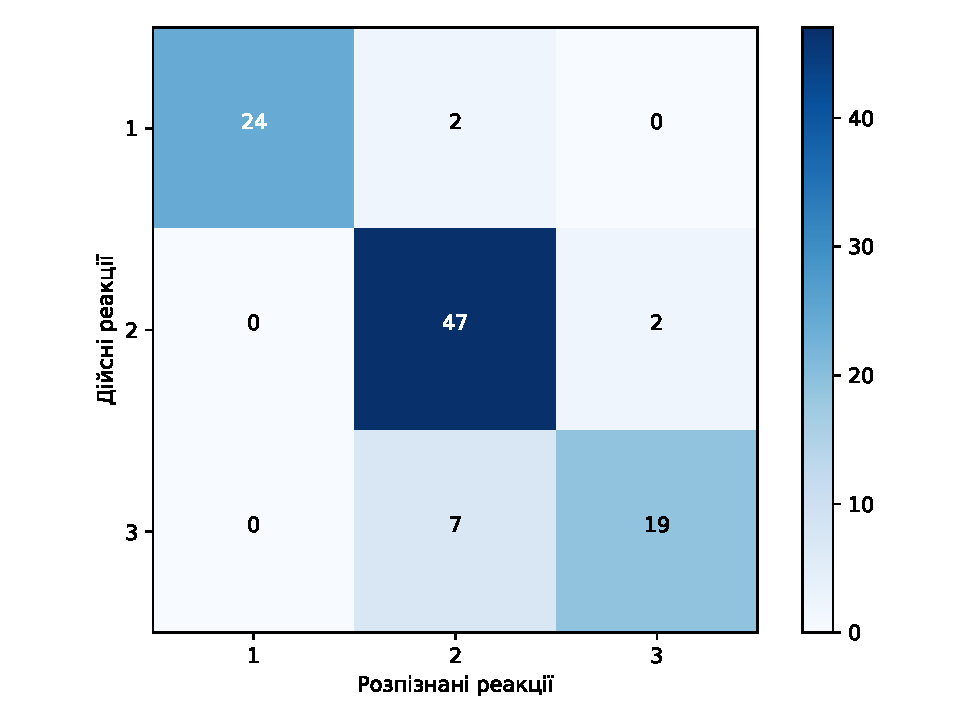
\includegraphics[width=0.3\linewidth]{confusion_matrix_data1_cnn_context_21}}
	
	\caption{Порівняння матриць помилок трьох різних методів (а, б, в) розпізнавання по реакціях для тестового контексту першого набору даних}
	\label{img:confusion_matrix_data1_context_21}
\end{figure}

Дослідивши матриці помилок моделювання інших контекстів (рис. \ref{img:confusion_matrix_data1_irs13_1} та \ref{img:confusion_matrix_data1_irs13_2}) методом інтелектуальних рефлекторних систем було виявлено, що моделі всіх контекстів в тій чи іншій мірі схильні до подібних помилок. Найменш схильними виявилися моделі контекстів 14, 16, 18 та 19, але за таблицею ми можемо бачити, що значення точності для цих контекстів менші за точність моделей для 13-го та тестового контекстів, де всі реакції були розпізнані як одна й та ж сама (рис. \ref{img:confusion_matrix_data1_irs13_context_21}).

Як кращі міри якості класифікаційної моделі для незбалансованих вибірок зазвичай використовують прецизійність (precision) та повноту (recall), які у випадку небінарної класифікації можуть бути визначені лише для певного класу, а не для моделі в цілому \cite{Powers_2011}. Для оцінки якості моделі було використано середні показники прецизійності та повноти по всім реакціям, що можуть бути визначені по формулам:

\begin{equation}
\label{eq:рrecision}
P=\frac{1}{n}\sum\limits_i\frac{TP_i}{TP_i+FP_i};
\end{equation}

\begin{equation}
\label{eq:recall}
R=\frac{1}{n}\sum\limits_i\frac{TP_i}{TP_i+FN_i},
\end{equation}

де $P$ --- середня прецизійність, $R$ --- середня повнота, $n$ --- кількість класів, $TP_i$ --- кількість вірно розпізнаних (True positive) зразків реакції $i$, $FP_i$ --- кількість зразків хибно розпізнаних (False positive) як реакція $i$, a $FN_i$ -- кількість зразків реакції $i$, хибно розпізнаних (False negative) як інша реакція.

Оскільки прецизійність показує лише помилки першого роду, а повнота лише помилки другого роду, існує узагальнена F-міра (F1, F-score) \cite{Powers_2011,Sasaki_2007}, що враховує обидва типи помилок як середньо-гармонічне, та може бути визначена за формулою:

\begin{equation}
\label{eq:f1}
F_1 = 2 \cdot \frac{P \cdot R}{P + R},
\end{equation}

де $F_1$ --- F-міра, $P$ --- прецизійність а $R$ --- повнота.

Дослідивши значення F-міри з таблиці \ref{tbl:total_data1_irs13} ми бачимо, що саме моделі контекстів 14, 16, 18 та 19, які виглядають найкраще на матрицях помилок, мають одні з найбільших значень F-міри, та порівняні зі значеннями моделей контекстів 1 та 2, що складаються лише з двох реакцій. Моделювання методом ІРС з розміром N-грам 2–4 (табл. \ref{tbl:total_data1_irs24}) показало схожі результати і дало невеликий приріст. якості розпізнавання, але цієї якості все одно недостатньо для практичного застосування моделі.

Метод згорткових нейронних мереж показав кращий результат. З таблиці \ref{tbl:total_data1_cnn} видно, що значення F-міри не набагато нижчі за точність, з чого можна зробити висновок, що ця модель краще працює з незбалансованими вибірками.

Для розрахунку показників у таблицях \ref{tbl:total_data1_irs13}--\ref{tbl:total_data1_cnn} використовувався метод кросс-валідації \cite{Kohavi_1995} з розбиттям повної вибірки на 5 рівних випадкових частин. Таким чином моделювання проводилося 5 разів, так, щоб кожна з 5 частин один раз була використана як тестова вибірка, а 4 інших частини в кожному моделюванні складали навчальну вибірку. Саме комбінація результатів на тестовій вибірці з 5-ти моделювань і була використана для розрахунку метрик в таблицях.

Розрахунок метрик на тестових вибірках показував точність розпізнавання від 90\% до 100\%, це свідчить про ефект перенавчання системи. Одним зі способів вирішення проблеми перенавчання є збільшення кількості даних. Було висунуто гіпотезу про низьку якість розпізнавання в звʼязку з недостатньою кількістю вхідних даних.

Отже, було вирішено провести другий етап дослідження, для якого було необхідно зібрати більшу кількість голосових даних. Для перевірки гіпотези вирішено зібрати голосові зразки лише для одного тестового контексту.

Додаткові голосові дані зібрано для одного контексту: 1 пристрій, 1 диктор (чоловік), 37 варіантів стимулів, 3 реакції у контексті, тобто 938 зразків.

Результати моделювання другого набору даних трьома різними методами ми можемо бачити в таблиці \ref{tbl:total_data2_irs13}, а матриці помилок зображено на рисунку \ref{img:confusion_matrix_data2_context_21}.

\begin{mytable}{ | c | c | c | c | }%
	{Порівняння якості розпізнавання другого набору даних різними методами}%
	{\label{tbl:total_data2_irs13}}%
	{ Показник & ІРС 1--3 & ІРС 2--4 & ЗНМ }		
	
	Точність розпізнання & 0.258 & 0.598 & 0.935 \\
	\hline
	Середня прецизійність & 0.226 & 0.636 & 0.939 \\
	\hline
	Середня повнота & 0.238 & 0.579 & 0.935 \\
	\hline
	Середня F-міра & 0.217 & 0.583 & 0.937 \\
	\hline
	Кількість & 925 & 925 & 925 \\
\end{mytable}

\begin{figure}[ht!]
	\centering
	\subbottom[Метод ІРС розміром 1--3 \label{img:confusion_matrix_data2_irs13_context_21}]{%
		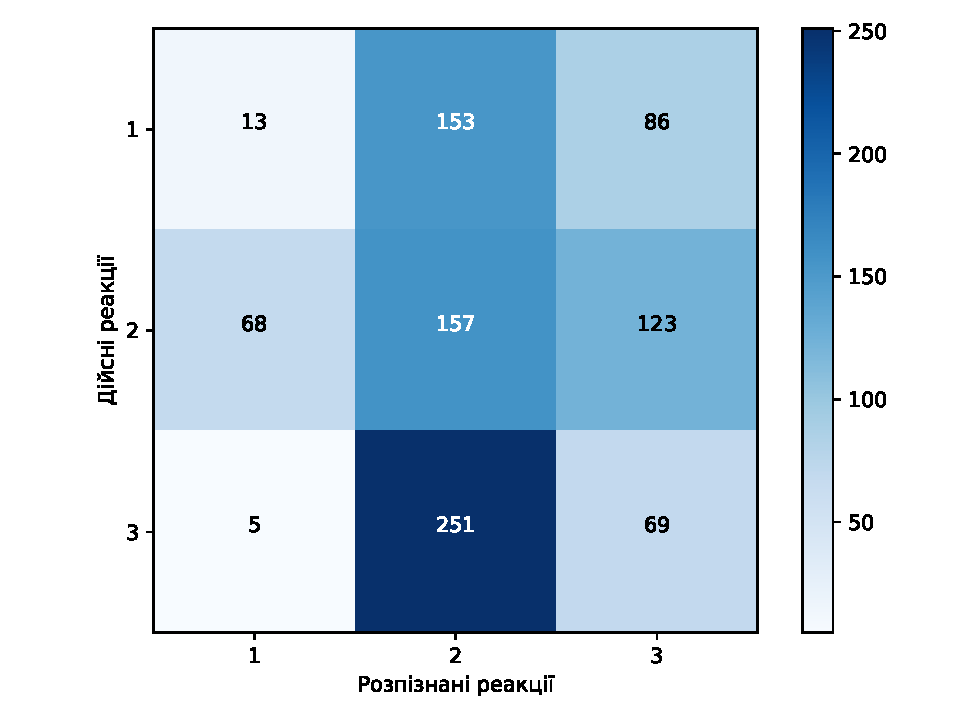
\includegraphics[width=0.3\linewidth]{confusion_matrix_data2_irs13_context_21}}
	\subbottom[Метод ІРС розміром 2--4 \label{img:confusion_matrix_data2_irs24_context_21}]{%
		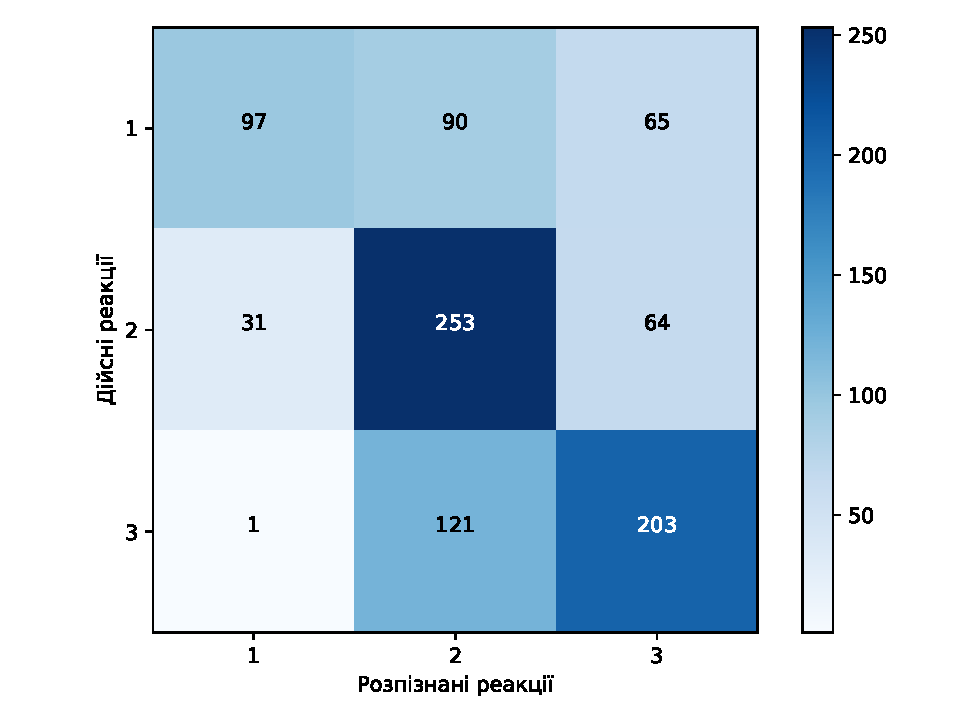
\includegraphics[width=0.3\linewidth]{confusion_matrix_data2_irs24_context_21}}
	\subbottom[Метод ЗНМ \label{img:confusion_matrix_data2_cnn_context_21}]{%
		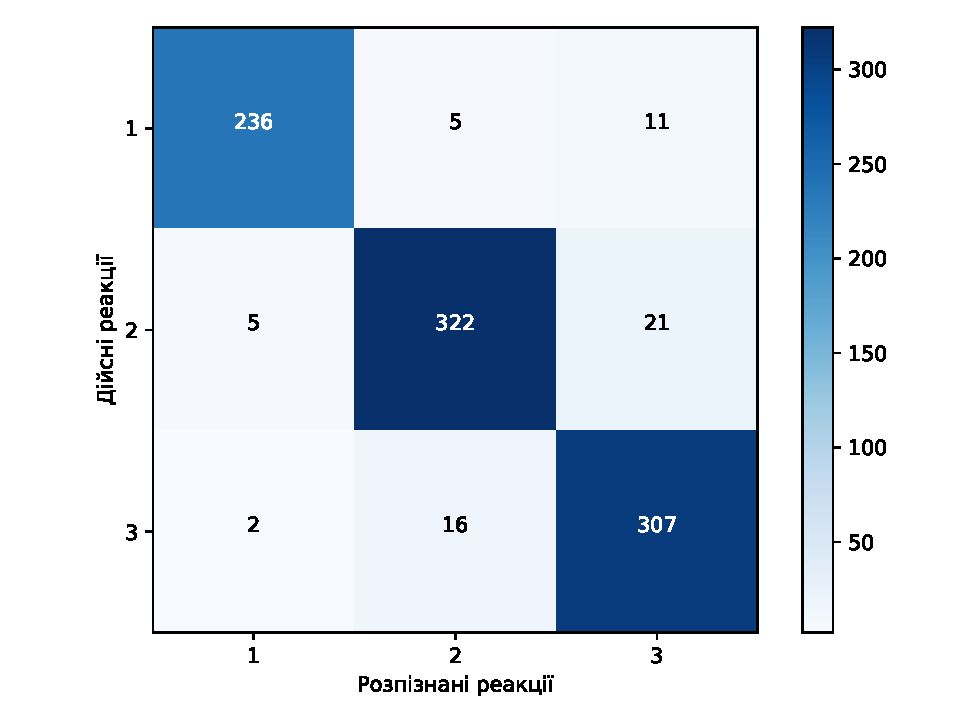
\includegraphics[width=0.3\linewidth]{confusion_matrix_data2_cnn_context_21}}
	
	\caption{Порівняння матриць помилок трьох різних методів (а, б, в) розпізнавання по реакціях для тестового контексту другого набору даних}
	\label{img:confusion_matrix_data2_context_21}
\end{figure}

З результатів моделювання можна бачити, що збільшення кількості вхідних даних безумовно покращило якість розпізнавання, для всіх методів. Моделювання інтелектуальними рефлекторними системами для одного контексту з великою вибіркою даних дало майже 60\% точності та значення F-міри 0.58. З матриці помилок (рис. \ref{img:confusion_matrix_data2_irs24_context_21}) не має явного переважання певної реакції над іншими. На жаль, отриманих значень точності досі недостатньо для успішного використання моделі на практиці. 

Моделювання методом згорткових нейронних мереж дало трохи більше 90\% точності та відповідне значення F-міри. Така точність є достатньою для практичного застосування, отже можна зробити висновок, що за даних умов дуальна система класифікації фонемної репрезентації голосових команд працює краще з використанням методу згорткових нейронних мереж для побудови моделі формалізації голосової інформації в системах диспетчеризації автотранспорту.

З цього можна бачити, що за даних умов, ефективність методу згорткових нейронних мереж вища за метод інтелектуальних рефлекторних систем більш ніж на 30\%. Ці результати викликають певний подив, оскільки в попередніх дослідженнях \cite{Egorchenkov_2016,Teslia_2014,Teslia_2013} метод інтелектуальних рефлекторних систем давав набагато кращі результати. Візуально дослідивши фонемну репрезентацію даних, ми помітили сильну зашумленість фонемних даних, хоча в звукових файлах рівень шуму був нижчим. Одне з можливих пояснень цього полягає в тому, що фонемний стенограф не був налаштований на використання мікрофону в мобільному телефоні, частотні показники якого можуть вносити перешкоди в роботу системи.  

\begin{mytable}[b!]{ | c | c | c | c | c | c | }%
	{Результати моделювання третього набору даних використовуючи ІРС з послідовностями розміром 1--3}%
	{\label{tbl:total_data3_irs13}}%
	{№ Контексту & \specialcell{3cm}{Точність \\ розпізнання} & \specialcell{3cm}{Середня \\ прецизійність} & \specialcell{3cm}{Середня \\ повнота} & \specialcell{3cm}{Середня \\ F-міра} & Кількість}	
	
	1 & 0.820 & 0.825 & 0.820 & 0.819 & 100 \\
\hline
3 & 0.637 & 0.660 & 0.637 & 0.611 & 350 \\
\hline
4 & 0.710 & 0.799 & 0.710 & 0.709 & 200 \\
\hline
5 & 0.630 & 0.714 & 0.630 & 0.633 & 300 \\
\hline
6 & 0.625 & 0.704 & 0.625 & 0.620 & 200 \\
\hline
7 & 0.524 & 0.563 & 0.524 & 0.528 & 500 \\
\hline
8 & 0.667 & 0.805 & 0.667 & 0.671 & 300 \\
\hline
9 & 0.660 & 0.790 & 0.660 & 0.667 & 250 \\
\hline
10 & 0.696 & 0.800 & 0.696 & 0.700 & 250 \\
\hline
11 & 0.608 & 0.703 & 0.608 & 0.600 & 250 \\
\hline
12 & 0.498 & 0.543 & 0.498 & 0.495 & 450 \\
\hline
13 & 0.700 & 0.697 & 0.700 & 0.698 & 150 \\
\hline
14 & 0.483 & 0.637 & 0.483 & 0.496 & 300 \\
\hline
15 & 0.597 & 0.664 & 0.597 & 0.587 & 300 \\
\hline
16 & 0.652 & 0.744 & 0.652 & 0.647 & 250 \\
\hline
17 & 0.431 & 0.495 & 0.431 & 0.430 & 350 \\
\hline
18 & 0.616 & 0.703 & 0.616 & 0.608 & 250 \\
\hline
19 & 0.595 & 0.713 & 0.595 & 0.596 & 200 \\
\hline
\specialcell{3cm}{По всій \\ вибірці} & 0.301 & 0.401 & 0.301 & 0.313 & 3200 \\
\hline
\specialcell{3cm}{Тестовий \\ контекст} & 0.733 & 0.738 & 0.733 & 0.734 & 150 \\
\end{mytable}

Далі, також, була висунута наступна гіпотеза про недостатню якість вхідних голосових даних: втраті деяких діапазонів частот при записі на мобільному пристрої та погано вплинуло на роботу фонемного стенографа. Були зібрані додаткові голосові дані на ПК за допомогою якісного USB мікрофона і з використанням функції запису додатку фонемного стенографа, як і в оригінальній роботі\cite{Teslia_2014}: 1 пристрій, 1 диктор (чоловік), 298 варіантів стимулів, 64 реакції, 3200 зразків. Результати досліджень при апробації засобів формалізації голосової інформації в системах диспетчерського контролю за рухом автотранспорту за пристроями приведені в табл. \ref{tbl:total_data3_irs13}, \ref{tbl:total_data3_irs24} та \ref{tbl:total_data3_cnn}.

\begin{mytable}{ | c | c | c | c | c | c | }%
	{Результати моделювання третього набору даних використовуючи ІРС з послідовностями розміром 2--4}%
	{\label{tbl:total_data3_irs24}}%
	{№ Контексту & \specialcell{3cm}{Точність \\ розпізнання} & \specialcell{3cm}{Середня \\ прецизійність} & \specialcell{3cm}{Середня \\ повнота} & \specialcell{3cm}{Середня \\ F-міра} & Кількість}	
	
	1 & 0.850 & 0.616 & 0.567 & 0.590 & 100 \\
\hline
3 & 0.866 & 0.883 & 0.866 & 0.862 & 350 \\
\hline
4 & 0.870 & 0.898 & 0.870 & 0.867 & 200 \\
\hline
5 & 0.830 & 0.863 & 0.830 & 0.830 & 300 \\
\hline
6 & 0.835 & 0.876 & 0.835 & 0.829 & 200 \\
\hline
7 & 0.774 & 0.795 & 0.774 & 0.775 & 500 \\
\hline
8 & 0.857 & 0.882 & 0.857 & 0.851 & 300 \\
\hline
9 & 0.884 & 0.763 & 0.737 & 0.737 & 250 \\
\hline
10 & 0.864 & 0.895 & 0.864 & 0.865 & 250 \\
\hline
11 & 0.824 & 0.852 & 0.824 & 0.814 & 250 \\
\hline
12 & 0.751 & 0.780 & 0.751 & 0.753 & 450 \\
\hline
13 & 0.813 & 0.655 & 0.610 & 0.620 & 150 \\
\hline
14 & 0.730 & 0.788 & 0.730 & 0.734 & 300 \\
\hline
15 & 0.780 & 0.824 & 0.780 & 0.778 & 300 \\
\hline
16 & 0.840 & 0.865 & 0.840 & 0.832 & 250 \\
\hline
17 & 0.646 & 0.692 & 0.646 & 0.641 & 350 \\
\hline
18 & 0.740 & 0.803 & 0.740 & 0.739 & 250 \\
\hline
19 & 0.825 & 0.853 & 0.825 & 0.821 & 200 \\
\hline
\specialcell{3cm}{По всій \\ вибірці} & 0.637 & 0.676 & 0.627 & 0.628 & 3200 \\
\hline
\specialcell{3cm}{Тестовий \\ контекст} & 0.893 & 0.895 & 0.893 & 0.894 & 150 \\
\end{mytable}

\begin{mytable}{ | c | c | c | c | c | c | }%
	{Результати моделювання третього набору даних використовуючи ЗНМ з послідовностями розміром 2--4}%
	{\label{tbl:total_data3_cnn}}%
	{№ Контексту & \specialcell{3cm}{Точність \\ розпізнання} & \specialcell{3cm}{Середня \\ прецизійність} & \specialcell{3cm}{Середня \\ повнота} & \specialcell{3cm}{Середня \\ F-міра} & Кількість}	
	
	1 & 0.900 & 0.901 & 0.900 & 0.900 & 100 \\
\hline
3 & 0.997 & 0.997 & 0.997 & 0.997 & 350 \\
\hline
4 & 0.990 & 0.990 & 0.990 & 0.990 & 200 \\
\hline
5 & 0.967 & 0.967 & 0.967 & 0.966 & 300 \\
\hline
6 & 0.975 & 0.976 & 0.975 & 0.975 & 200 \\
\hline
7 & 0.948 & 0.950 & 0.948 & 0.948 & 500 \\
\hline
8 & 0.983 & 0.984 & 0.983 & 0.983 & 300 \\
\hline
9 & 0.976 & 0.976 & 0.976 & 0.976 & 250 \\
\hline
10 & 0.960 & 0.961 & 0.960 & 0.960 & 250 \\
\hline
11 & 0.952 & 0.956 & 0.952 & 0.951 & 250 \\
\hline
12 & 0.951 & 0.952 & 0.951 & 0.950 & 450 \\
\hline
13 & 0.927 & 0.926 & 0.927 & 0.926 & 150 \\
\hline
14 & 0.950 & 0.950 & 0.950 & 0.950 & 300 \\
\hline
15 & 0.923 & 0.925 & 0.923 & 0.922 & 300 \\
\hline
16 & 0.968 & 0.971 & 0.968 & 0.968 & 250 \\
\hline
17 & 0.951 & 0.954 & 0.951 & 0.952 & 350 \\
\hline
18 & 0.928 & 0.929 & 0.928 & 0.928 & 250 \\
\hline
19 & 0.980 & 0.981 & 0.980 & 0.980 & 200 \\
\hline
\specialcell{3cm}{По всій \\ вибірці} & 0.890 & 0.891 & 0.890 & 0.890 & 3200 \\
\hline
\specialcell{3cm}{Тестовий \\ контекст} & 0.973 & 0.974 & 0.973 & 0.973 & 150 \\
\end{mytable}

Побудувавши графіки розподілу точності та F-міри від кількості зразків у контексті (рис. \ref{img:accuracy_distribution_data3}) ми можемо бачити, що прямої залежності немає. Але на якість розпізнавання повинна впливати кількість реакцій в контексті і середня кількість записів зразків голосових даних на кожну реакцію.

\begin{figure}[!t]
	\centering
	\subbottom[Метод ІРС розміром 1--3 \label{img:accuracy_distribution_data3_irs13}]{%
		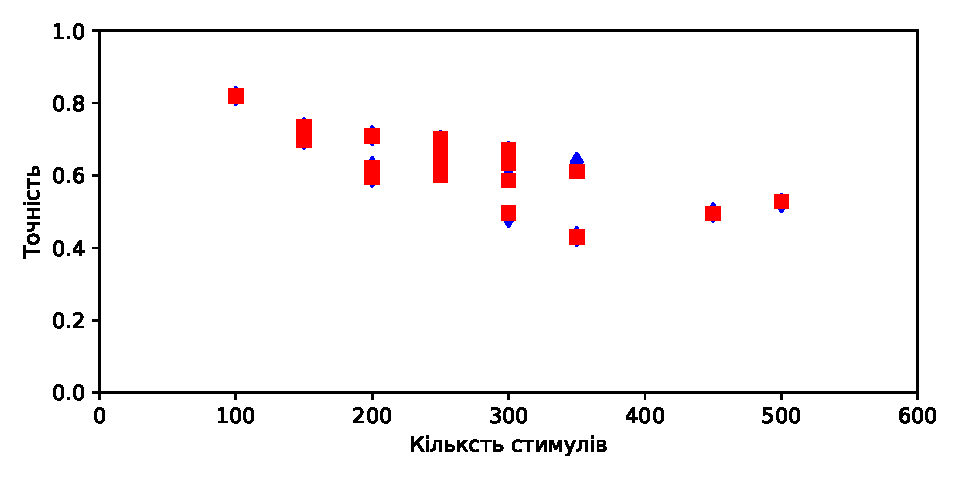
\includegraphics[width=.7\linewidth]{accuracy_distribution_data3_irs13}}
	\\
	\subbottom[Метод ІРС розміром 2--4 \label{img:accuracy_distribution_data3_irs24}]{%
		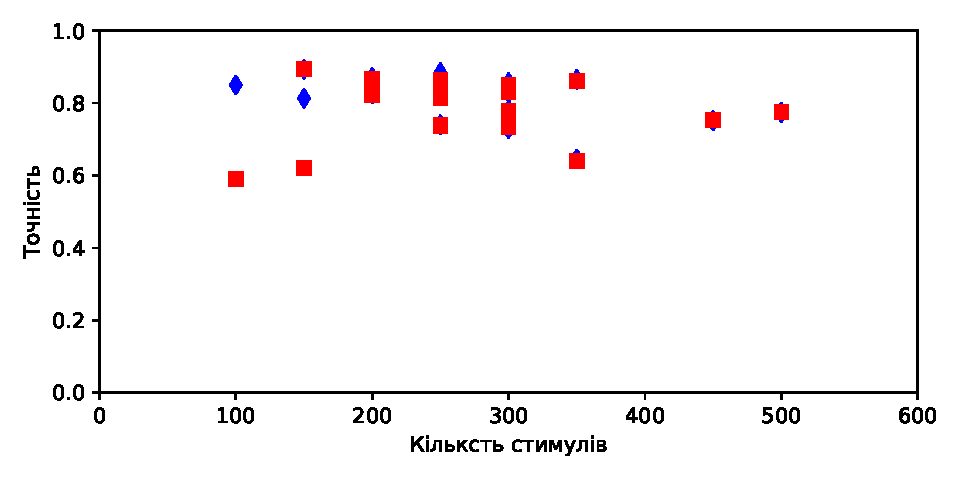
\includegraphics[width=.7\linewidth]{accuracy_distribution_data3_irs24}}
	\\
	\subbottom[Метод ЗНМ \label{img:accuracy_distribution_data3_cnn}]{%
		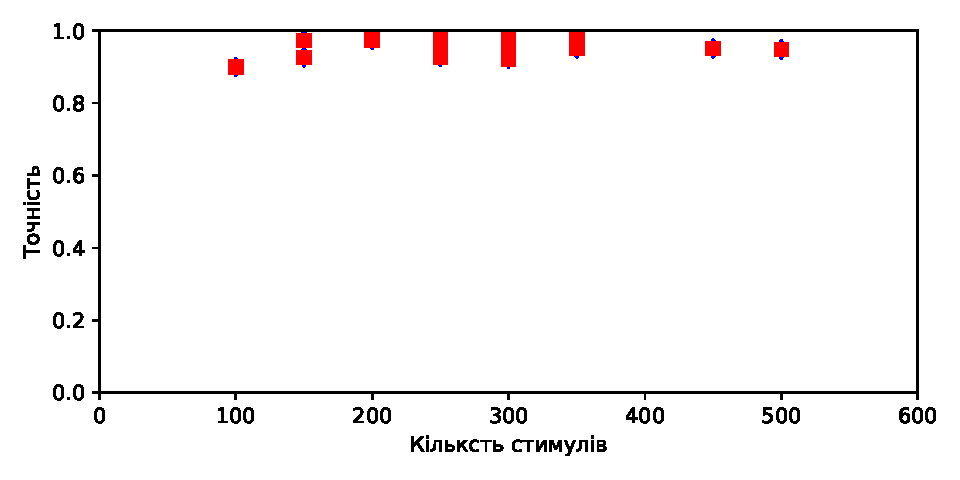
\includegraphics[width=.7\linewidth]{accuracy_distribution_data3_cnn}}
	\caption{Розподіл точності (червоні квадрати) та F-міри (сині ромби) за кількістю голосових зразків при моделюванні контекстів третього набору даних різними методами}
	\label{img:accuracy_distribution_data3}
\end{figure}

З матриці помилок моделювання тестового контексту різними методами (рис. \ref{img:confusion_matrix_data3_context_21}), ми можемо бачити, що всі методи показують ницький рівень помилок розпізнавання.

\begin{figure}
	\centering
	\subbottom[Метод ІРС розміром 1--3 \label{img:confusion_matrix_data3_irs13_context_21}]{%
		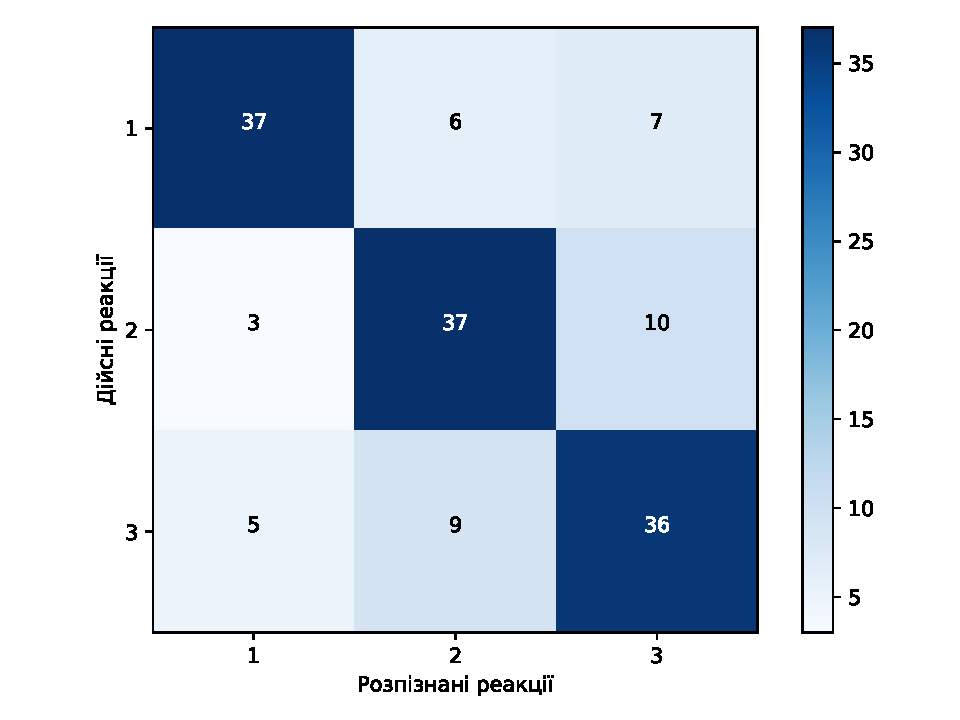
\includegraphics[width=0.3\linewidth]{confusion_matrix_data3_irs13_context_21}}
	\subbottom[Метод ІРС розміром 2--4 \label{img:confusion_matrix_data3_irs24_context_21}]{%
		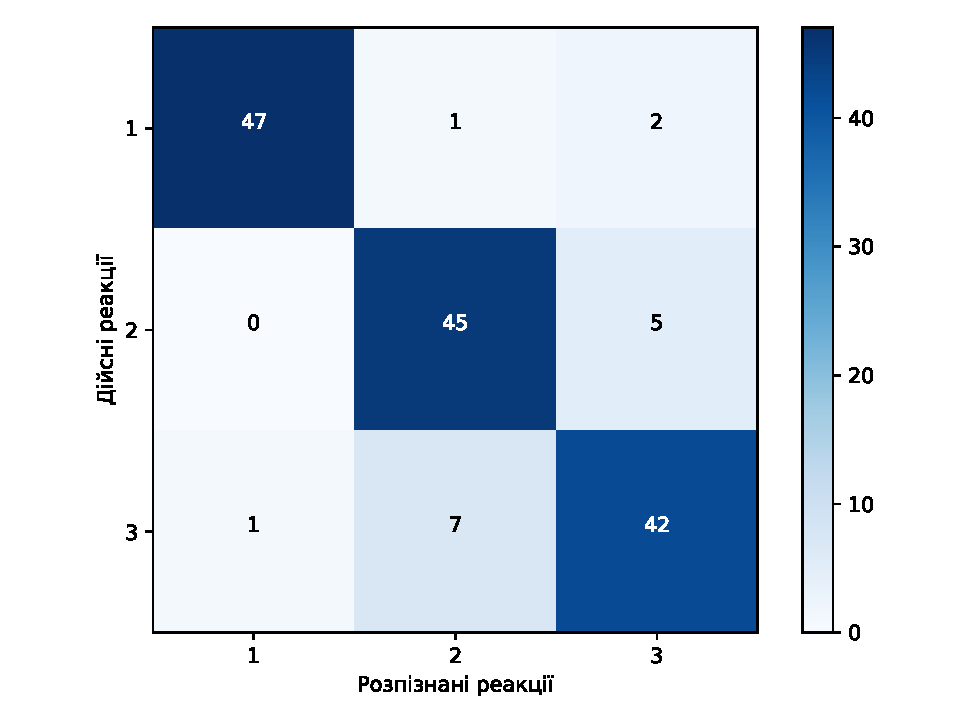
\includegraphics[width=0.3\linewidth]{confusion_matrix_data3_irs24_context_21}}
	\subbottom[Метод ЗНМ \label{img:confusion_matrix_data3_cnn_context_21}]{%
		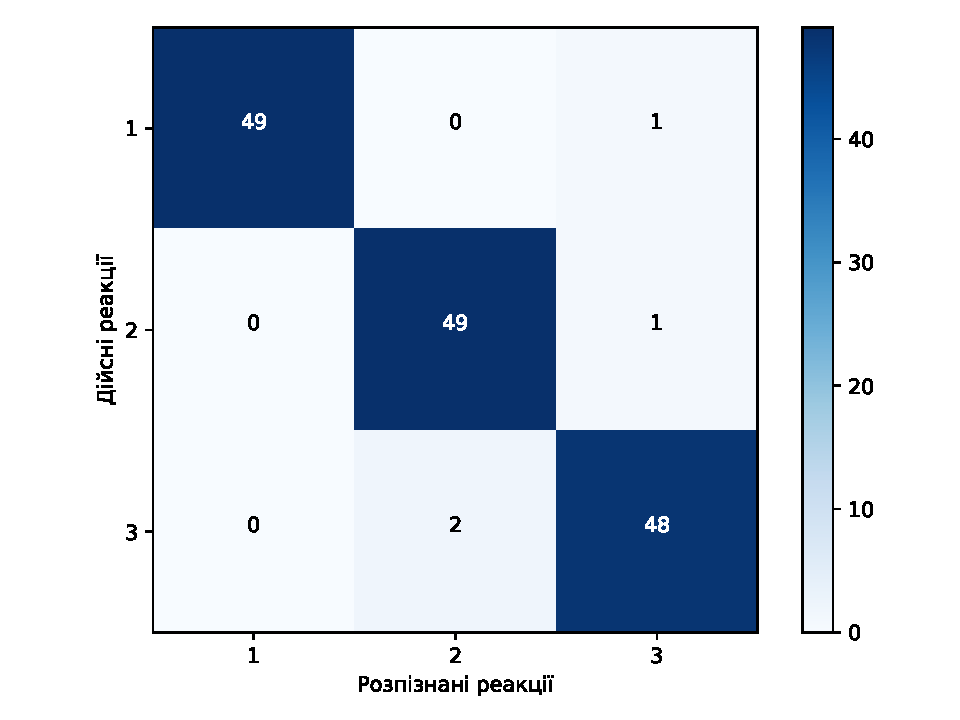
\includegraphics[width=0.3\linewidth]{confusion_matrix_data3_cnn_context_21}}
	
	\caption{Порівняння матриць помилок трьох різних методів розпізнавання по реакціях для тестового контексту третього набору даних}
	\label{img:confusion_matrix_data3_context_21}
\end{figure}

Порівнюючи дані розподілів, що приведені на рис. \ref{img:accuracy_distribution_data1} та \ref{img:accuracy_distribution_data3} можемо твердити про те, що з підвищенням загальної кількості стимулів відбувається зріст розпізнаних стимулів, що призводить до збільшення точності розпізнання при апробації засобів формалізації голосової інформації в системах диспетчерського контролю за рухом автотранспорту.

Моделювання рефлекторними системами при апробації засобів формалізації голосової інформації в системах диспетчерського контролю за рухом автотранспорту для одного контексту дало близько 80\% точності (табл. \ref{tbl:total_data3_irs13}, \ref{tbl:total_data3_irs24}). Моделювання нейронною мережею майже не дало приросту в розпізнаванні, що свідчить про ефективність навчання згорткових фільтрів порівняно з попередньою обробкою.

Перевірка моделювання розпізнавання команд на основі ітеративного процесу збору даних та введення нових критеріїв оцінки, якщо попередні не дали достатньої точності оцінювання, може забезпечити процес порівняння ефективності різних методів класифікації в дуальній моделі формалізації голосової взаємодії.

Доцільно використовувати набір метрик оцінки ефективності моделей класифікації, що обовʼязково має включати крім оцінки точності ще робастні метрики для незбалансованої вибірки (такі, як прецизійність, повноту, F-міру) або візуальний аналіз матриць помилок. 

Досягнуто прийнятний для практичного використання рівень точності в моделі, побудованої методом згорткових нейронних мереж при другій ітерації моделювання з достатньою кількістю навчальних даних.

Для апробації розроблених засобів, систему підтримки диспетчеризації автотранспорту (підрозділ \ref{sect2_2}) було впроваджено на підприємстві ТОВ «Українські Інформаційні Технології» \cite{SngTrans} та досліджено її використання протягом року у трьох підприємствах-клієнтах.

Результати цієї апробації показали загальне підвищення ефективності процесу доставки на 14.5\%, за рахунок скорочення кількості необхідних транспортних засобів на 7.1\% та підвищення кількості точок які можуть бути обслуговуванні одним транспортним засобом в середньому на 9.4\%.

При цьому дослідження показали, що в залежності від навантаженості доби, від 5\% до 15\% точок доставки повʼязані з певними інцидентами та відхиленнями від плану, і лише 10\% з цих інцидентів вдається ліквідувати або надолужити. Статистичне моделювання проведене на основі порівняння поведінки різних водіїв показало, що водії які вчасно повідомляють про можливі інциденти через додаток з сенсорним управлінням можуть уникнути чи виправити до 50\% інцидентів, а отже запровадження голосового інтерфейсу може розповсюдити ці результати на всіх водіїв \cite{SngTrans}.

\section*{Висновки до розділу 4}
\addcontentsline{toc}{section}{Висновки до розділу 4}

1. Розроблений засіб формалізації голосової інформації дозволяє водію не відволікатись від управління автомобілем і слідкувати за дорожніми умовами та обстановкою, що дає змогу прискорити доставку продукції в процесі дистрибуції, а також підвищити рівень безпеки.

2. Розглянуті особливості використання розроблених засобів формалізації голосової інформації в системах диспетчерського контролю за рухом автотранспорту показали, що водію автомобіля, який буде здійснювати доставку продукції в процесі дистрибуції і вперше зіштовхнеться із засобом формалізації голосової інформації, що діє в рамках системи диспетчерського контролю за рухом автотранспорту, необхідно попередньо перевірити і при потребі донавчити систему розпізнавати його голосові команди з відповідних контекстів.

3. Перевірка моделювання розпізнавання команд на основі ітеративного процесу збору даних та введення нових критеріїв оцінки, якщо попередні не дали достатньої точності оцінювання, може забезпечити процес порівняння ефективності різних методів класифікації в дуальній моделі формалізації голосової взаємодії.
Використано розширений набір метрик оцінки ефективності моделей класифікації, що включав крім оцінки точності ще робастні метрики для незбалансованої вибірки (прецизійність, повноту, F-міру) та візуальний аналіз матриць помилок.

4. Оцінка ефективності дуальної системи формалізації голосової інформації проведена експериментальним шляхом у три етапи: на першому етапі первинного моделювання виявлено необхідність збільшення кількості вхідних даних; на другому перевірено гіпотезу недостатності кількості вхідних даних; на третьому --- гіпотезу недостатньої якості звукового сигналу. Прийнятний для практичного використання рівень точності в моделі, побудованій методом згорткових нейронних мереж досягнуто на другому етапі моделювання, а в моделі, побудованій методом інтелектуальних рефлекторних систем --- на третьому.

5. Впровадження протягом року у трьох дистрибуційних компаніях підтвердило ефективність розробленої інформаційної технології формалізації голосової інформації: система підтримки диспетчеризації автотранспорту підвищує загальну ефективність процесу доставки за рахунок скорочення кількості необхідних транспортних засобів та підвищення кількості точок які можуть бути обслуговуванні одним транспортним засобом; запровадження голосового інтерфейсу може підвищити відсоток уникнення чи виправлення водіями інцидентів і відхилень від планового маршруту.

